This chapter provides a detailed, step-by-step blueprint of the research design and analytical framework used to compare the traditional and machine learning-based calibration methods. It begins by describing the dataset, including the source and specifications of the swaption and interest rate data. Subsequently, it outlines the data preprocessing pipeline, covering the bootstrapping of zero-coupon curves and the feature engineering process designed to capture key market dynamics. The core of the chapter details the architecture of the neural network model, the hyperparameter optimization strategy, and the implementation of the traditional Levenberg-Marquardt algorithm. Finally, it defines the specific metrics for accuracy, speed, and robustness that will be used to conduct a rigorous and objective evaluation of both approaches.

\subsection{Dataset}
\subsubsection{Time Period}
The market data used for the calibration of the one-factor Hull–White model covers a continuous time span of 92 calendar days, from June 1, 2025, to August 31, 2025. Observations are available for each calendar day within this period; weekends and public holidays are not excluded. The dataset therefore represents a high-frequency sample of daily market conditions. All market snapshots were collected at a daily frequency, ensuring a consistent temporal resolution across the entire observation window.

\subsubsection{Swaptions}
The calibration is based on a comprehensive panel of European at-the-money (ATM) payer and receiver swaptions quoted in the Euro (EUR) market. Each daily market snapshot consists of a complete normal volatility surface containing 228 distinct volatility points, derived from combinations of option maturities and underlying swap tenors.

The set of option maturities includes:
1 month, 3 months, 9 months, 1 year, 2 years, 3 years, 4 years, 5 years, 6 years, 7 years, 8 years, 9 years, 10 years, 12 years, 15 years, 20 years, 25 years, and 30 years.

The corresponding underlying swap tenors are:
1 year, 2 years, 3 years, 4 years, 5 years, 7 years, 10 years, 12 years, 15 years, 20 years, 25 years, and 30 years.

The floating leg of each underlying swap resets on a semiannual (6-month) basis. Volatilities are quoted in normal (Bachelier) terms, expressed in basis points (bps) of the underlying swap rate, and represent the mid-market levels (average of bid and ask quotes). Only ATM swaptions are considered in the calibration.

All swaption data were obtained from Bloomberg using the \texttt{VCUB} function with \texttt{BVOL} as the source. Due to the university's Bloomberg license restrictions, direct data downloads were not permitted; therefore, the data were captured via screenshots and subsequently converted into Excel format for processing. Bloomberg employs the EUR OIS (ESTR) discounting curve, identified as \texttt{(514) EUR OIS (ESTR)}, and the EUR swap curve \texttt{(45) Euro} for the construction of the volatility cube. This ensures internal consistency between the volatility and yield curve data used in the Hull–White model calibration.

\subsubsection{Swap Curves}
The initial yield curves employed for the Hull–White model calibration are derived from the EUR (vs. 6M EURIBOR) Swap / Projection Curve, identified in Bloomberg as \texttt{45}. This curve represents a forward (projection) curve used to generate 6-month EURIBOR forward rates for pricing and valuation. The discounting is performed using the EUR OIS (ESTR) curve (\texttt{Bloomberg ID 514}), consistent with the multi-curve framework applied in current market practice.

The market instruments used in the bootstrapping of the projection curve include:
\begin{itemize}
	\item Cash deposits: Overnight to 12-month maturities, anchoring the short end of the curve.
	\item Forward Rate Agreements (FRAs): Typically spanning 1×7 to 9×15 months, bridging the short and medium-term maturities.
	\item Interest-rate swaps: Par fixed-vs-6M EURIBOR swaps from 1 year up to 30 years, forming the long end of the term structure.
\end{itemize}

Day-count conventions follow market standards: ACT/360 for short and medium maturities and 30U/360 for the long end. All market quotes correspond to mid (bid/ask midpoint) levels. The market data source is the Bloomberg Generic (BGN) composite, which aggregates dealer contributions to provide representative market levels.

The curve is bootstrapped sequentially from cash deposits through FRAs to interest-rate swaps, producing a continuous zero-rate and forward-rate term structure. The interpolation is typically performed in a log-linear fashion on either discount factors or zero rates. Within the Bloomberg volatility cube environment (\texttt{VCUB}), this curve appears as \texttt{Swap Curve (45) Euro} and provides consistent forward-rate inputs for the calibration of EUR 6M swaption volatilities.

\subsubsection{MOVE Index}
The MOVE index represents the Treasury market's implied volatility and serves as a primary external indicator of interest rate uncertainty. Daily open values of the MOVE index were collected from Yahoo Finance to capture the most up-to-date measure of market-implied interest rate volatility at the start of each trading day. By using the open rather than closing values, the neural network is able to predict Hull–White model parameters early in the day, leveraging the most recent available information without waiting for end-of-day data. The MOVE index is particularly relevant as it captures expected fluctuations in interest rates, which directly influence the calibration of the Hull–White model.

\subsubsection{VIX Index}
The VIX index provides a widely recognized measure of equity market implied volatility and serves as a general gauge of market fear and risk appetite. Daily open values of the VIX were downloaded from Yahoo Finance to reflect the initial market sentiment for each trading day. High VIX levels, indicative of a "risk-off" environment, can have spillover effects on bond and swap markets, thereby indirectly affecting European interest rates. Including VIX open values in the dataset allows the neural network to incorporate contemporaneous equity market volatility into the prediction of Hull–White parameters, potentially improving model responsiveness to market stress conditions.

\subsubsection{EUR/USD Exchange Rate}
The EUR/USD exchange rate reflects the relative economic and monetary conditions between the Eurozone and the United States. Daily open prices were obtained from Yahoo Finance to capture the most current cross-currency market information at the start of each trading day. Large movements in the EUR/USD rate may indicate capital flows or diverging monetary policy actions between the European Central Bank and the Federal Reserve, which have direct implications for European interest rates. By including the open EUR/USD rate in the feature set, the neural network can incorporate up-to-date FX market dynamics when predicting Hull–White model parameters.

\subsection{Descriptive Analysis of Market and Model Inputs}
This section provides a detailed examination of the key figures illustrating the underlying financial data and model inputs used in this study. Each figure is analyzed with respect to its economic interpretation and its implications for the modeling framework.

\begin{figure}[H]
	\centering
	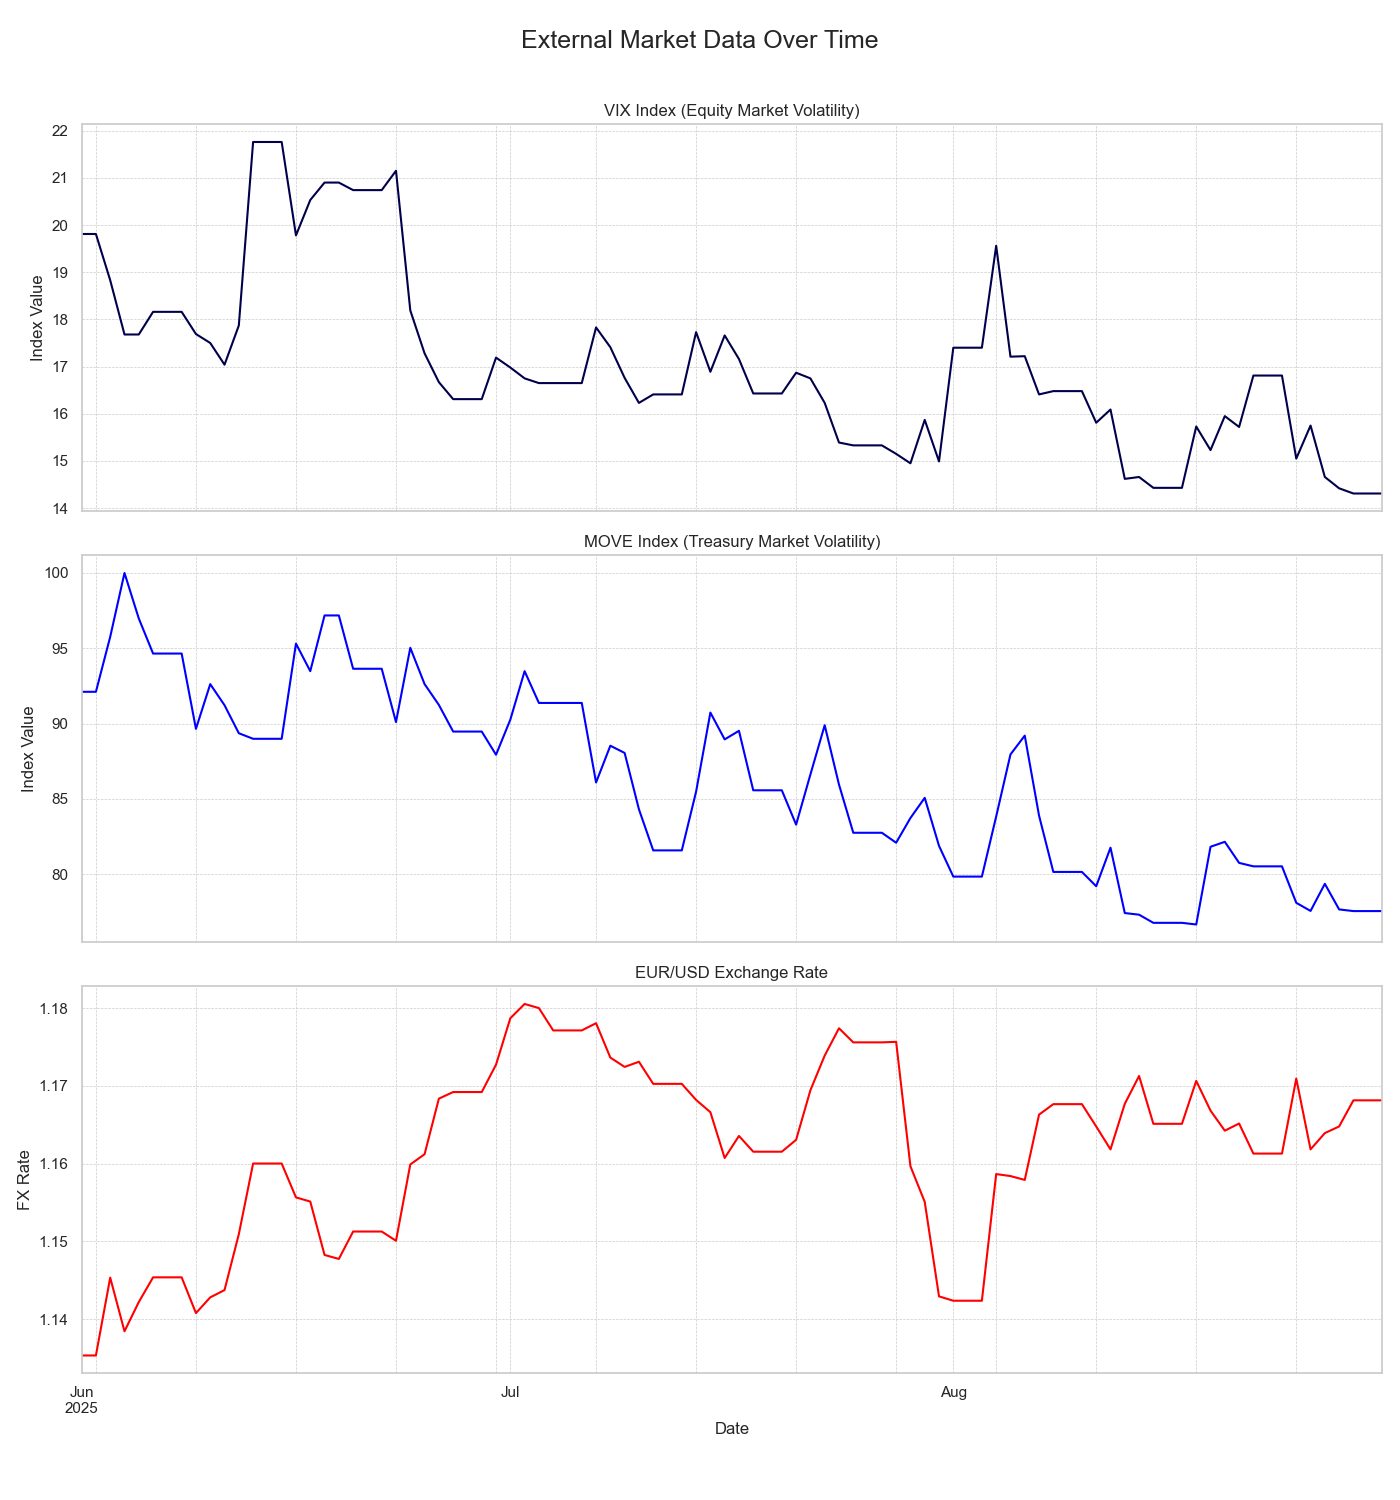
\includegraphics[width=1\textwidth]{images/descriptive_data_analysis/external_data_time_series.png}
	\caption{Time Series of Market-Wide Indicators (VIX, MOVE, and EUR/USD)}
	\label{fig:external_data_time_series}
\end{figure}

Figure~\ref{fig:external_data_time_series} depicts the evolution of key market indicators between June and late August 2025. The overall market environment during this period is characterized by a notable decrease in volatility across major asset classes. The \textit{VIX Index}, representing equity market volatility, begins near a relatively elevated level of 20 before declining sharply in late June and stabilizing within a range of 14–17. This pattern suggests a reduction in perceived equity market risk. Similarly, the \textit{MOVE Index}, a measure of Treasury market volatility, exhibits an even more pronounced decline—from approximately 100 to below 80—indicating a substantial calming of interest rate expectations. Concurrently, the \textit{EUR/USD} exchange rate shows a strengthening of the Euro against the U.S. Dollar, peaking near 1.18 in mid-July before a modest correction. These co-evolving patterns reflect a broad reduction in cross-asset risk and uncertainty.

% --- TABLE 1 INSERTED HERE ---
\begin{table}[H]
	\centering
	\begin{threeparttable}
		\caption{Summary Statistics of External Market Factors}
		\label{tab:external_summary}
		\begin{tabular}{lccccc}
			\toprule
			\textbf{Factor} & \textbf{Mean} & \textbf{Median} & \textbf{Std. Dev.} & \textbf{Skewness} & \textbf{Kurtosis} \\
			\midrule
			VIX Index       & 17.05         & 16.71           & 1.89               & 0.89              & 0.34              \\
			MOVE Index      & 86.29         & 86.02           & 6.12               & 0.10              & -1.10             \\
			EUR/USD Rate    & 1.162         & 1.164           & 0.011              & -0.57             & -0.54             \\
			\bottomrule
		\end{tabular}
		\begin{tablenotes}
			\footnotesize
			\item  A summary of the key external market factors over the analysis period. The positive skew in the VIX index and the non-zero kurtosis across all factors suggest deviations from a normal distribution.
		\end{tablenotes}
	\end{threeparttable}
\end{table}


Table~\ref{tab:external_summary} provides a quantitative summary of the external market factors depicted in Figure~\ref{fig:external_data_time_series}. The statistics confirm the visual analysis, detailing the central tendency and dispersion of each series. Notably, the VIX Index exhibits significant positive skewness (0.89), indicating that upward spikes in volatility are more pronounced than downward movements. Conversely, the EUR/USD rate shows a negative skew (-0.57). The kurtosis values, which deviate from the zero value of a mesokurtic distribution, provide further numerical evidence that these financial time series are not normally distributed, a crucial consideration for the modeling approach.

\begin{figure}[H]
	\centering
	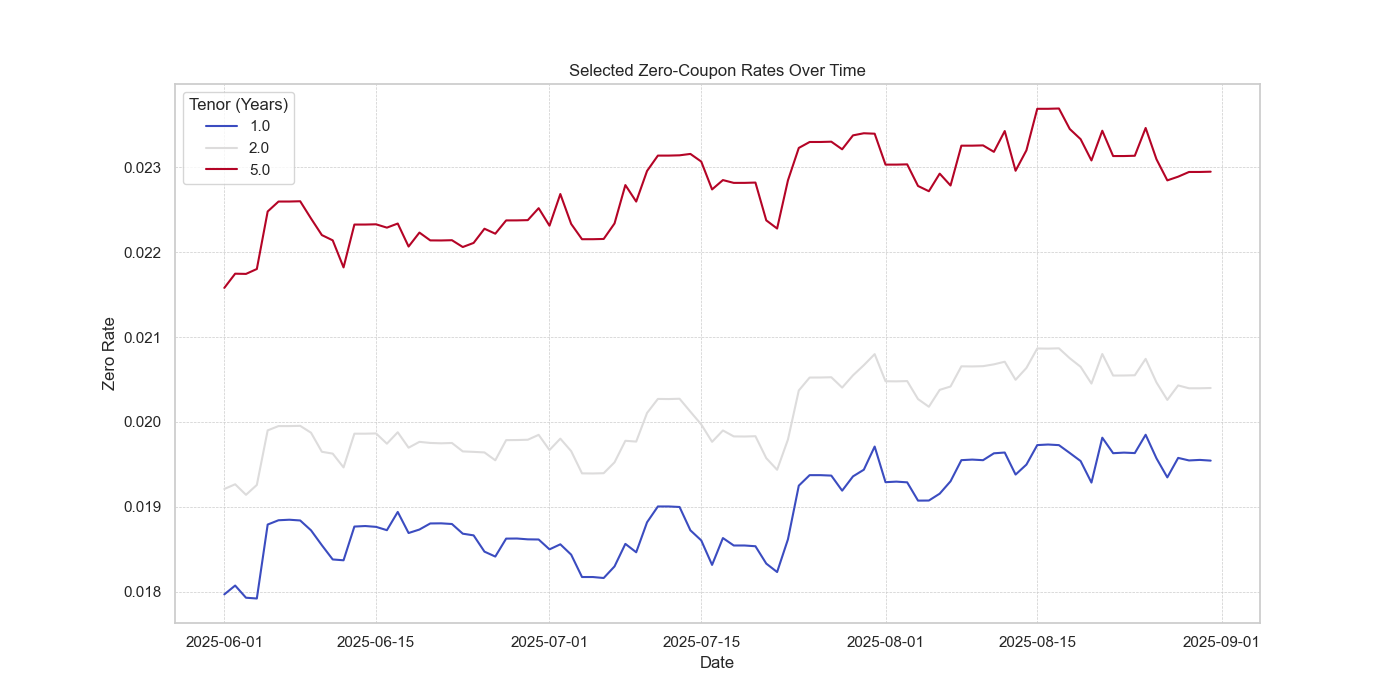
\includegraphics[width=1\textwidth]{images/descriptive_data_analysis/yield_curve_selected_tenors.png}
	\caption{Yield Curve Dynamics for Selected Tenors (1Y, 2Y, 5Y)}
	\label{fig:yield_curve_selected_tenors}
\end{figure}

Figure~\ref{fig:yield_curve_selected_tenors} illustrates the time series of yields across selected maturities. The yield curve retains its normal, upward-sloping shape throughout the observation window. A gradual upward shift is visible across all tenors, indicating a moderate tightening of monetary conditions. The largely parallel movement across maturities implies that changes are predominantly driven by a “level” factor. Minor deviations in spreads, however, suggest that “slope” and “curvature” components contribute modestly to the curve’s dynamics.

\begin{figure}[H]
	\centering
	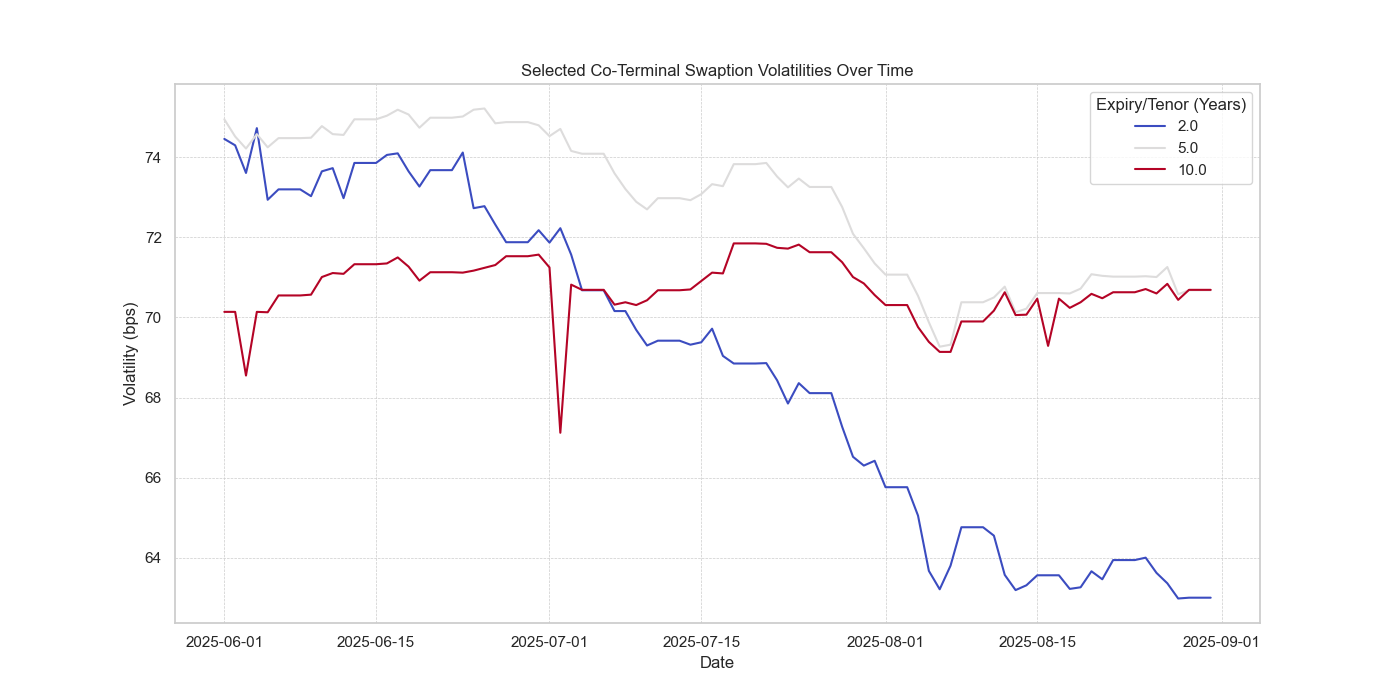
\includegraphics[width=1\textwidth]{images/descriptive_data_analysis/vol_surface_coterminal_series.png}
	\caption{Time Series of Co-Terminal Swaption Volatilities}
	\label{fig:vol_surface_coterminal_series}
\end{figure}

Figure~\ref{fig:vol_surface_coterminal_series} presents the evolution of the co-terminal swaption volatility term structure. The curve is generally downward sloping, with shorter maturities exhibiting higher volatility levels than longer maturities. The short-term (2-year) volatility declines sharply from over 74~bps to approximately 63~bps, whereas the long-term (10-year) volatility remains comparatively stable. This differential behavior leads to a pronounced flattening of the volatility term structure—a key empirical feature that any robust model should accurately capture.

\begin{figure}[H]
	\centering
	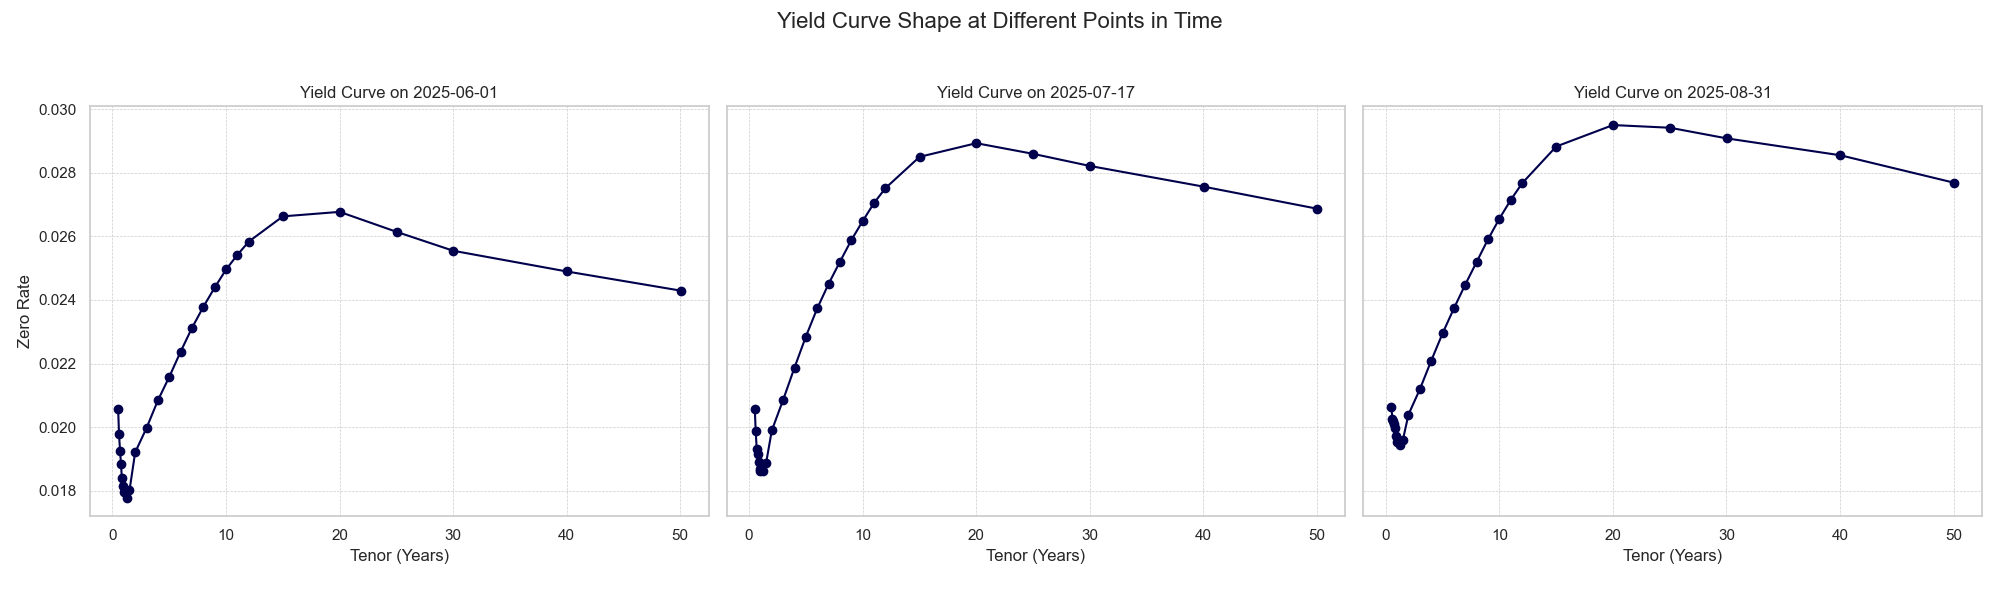
\includegraphics[width=1\textwidth]{images/descriptive_data_analysis/yield_curve_2d_snapshots.png}
	\caption{Yield Curve Snapshots over Time}
	\label{fig:yield_curve_2d_snapshots}
\end{figure}

Figure~\ref{fig:yield_curve_2d_snapshots} visualizes static yield curve snapshots at different points in time. The yield curve consistently displays a concave, upward-sloping shape, typical for stable economic environments. The entire curve shifts upward from June to August, reinforcing the observed trend of rising interest rates. Moreover, the curvature appears to increase slightly over time, suggesting subtle changes in the underlying term structure dynamics.

% --- TABLE 2 INSERTED HERE ---
\begin{table}[H]
	\centering
	\begin{threeparttable}
		\caption{Descriptive Statistics for Key Yield Curve Tenors}
		\label{tab:yield_curve_summary}
		\begin{tabular}{lcccc}
			\toprule
			\textbf{Tenor} & \textbf{Mean Rate (\%)} & \textbf{Std. Dev. (\%)} & \textbf{Skewness} & \textbf{Kurtosis} \\
			\midrule
			1-Year         & 1.90                    & 0.05                    & -0.02             & -1.10             \\
			5-Year         & 2.27                    & 0.05                    & -0.18             & -0.88             \\
			10-Year        & 2.62                    & 0.06                    & -0.25             & -1.04             \\
			30-Year        & 2.76                    & 0.12                    & -0.29             & -1.22             \\
			\bottomrule
		\end{tabular}
		\begin{tablenotes}
			\footnotesize
			\item  Descriptive statistics for selected benchmark tenors of the zero-coupon yield curve. Mean Rate and Standard Deviation are expressed in percentage points.
		\end{tablenotes}
	\end{threeparttable}
\end{table}


Table~\ref{tab:yield_curve_summary} quantifies the characteristics of the yield curve by presenting descriptive statistics for key benchmark tenors. The increasing mean rate with tenor numerically confirms the upward-sloping nature of the term structure. A particularly important finding is the behavior of the standard deviation, which increases from 0.05\% for the 1-year rate to 0.12\% for the 30-year rate. This demonstrates that the long end of the yield curve is substantially more volatile in absolute terms, a stylized fact that is further explored in Figure~\ref{fig:yield_curve_std_by_tenor}.

\begin{figure}[H]
	\centering
	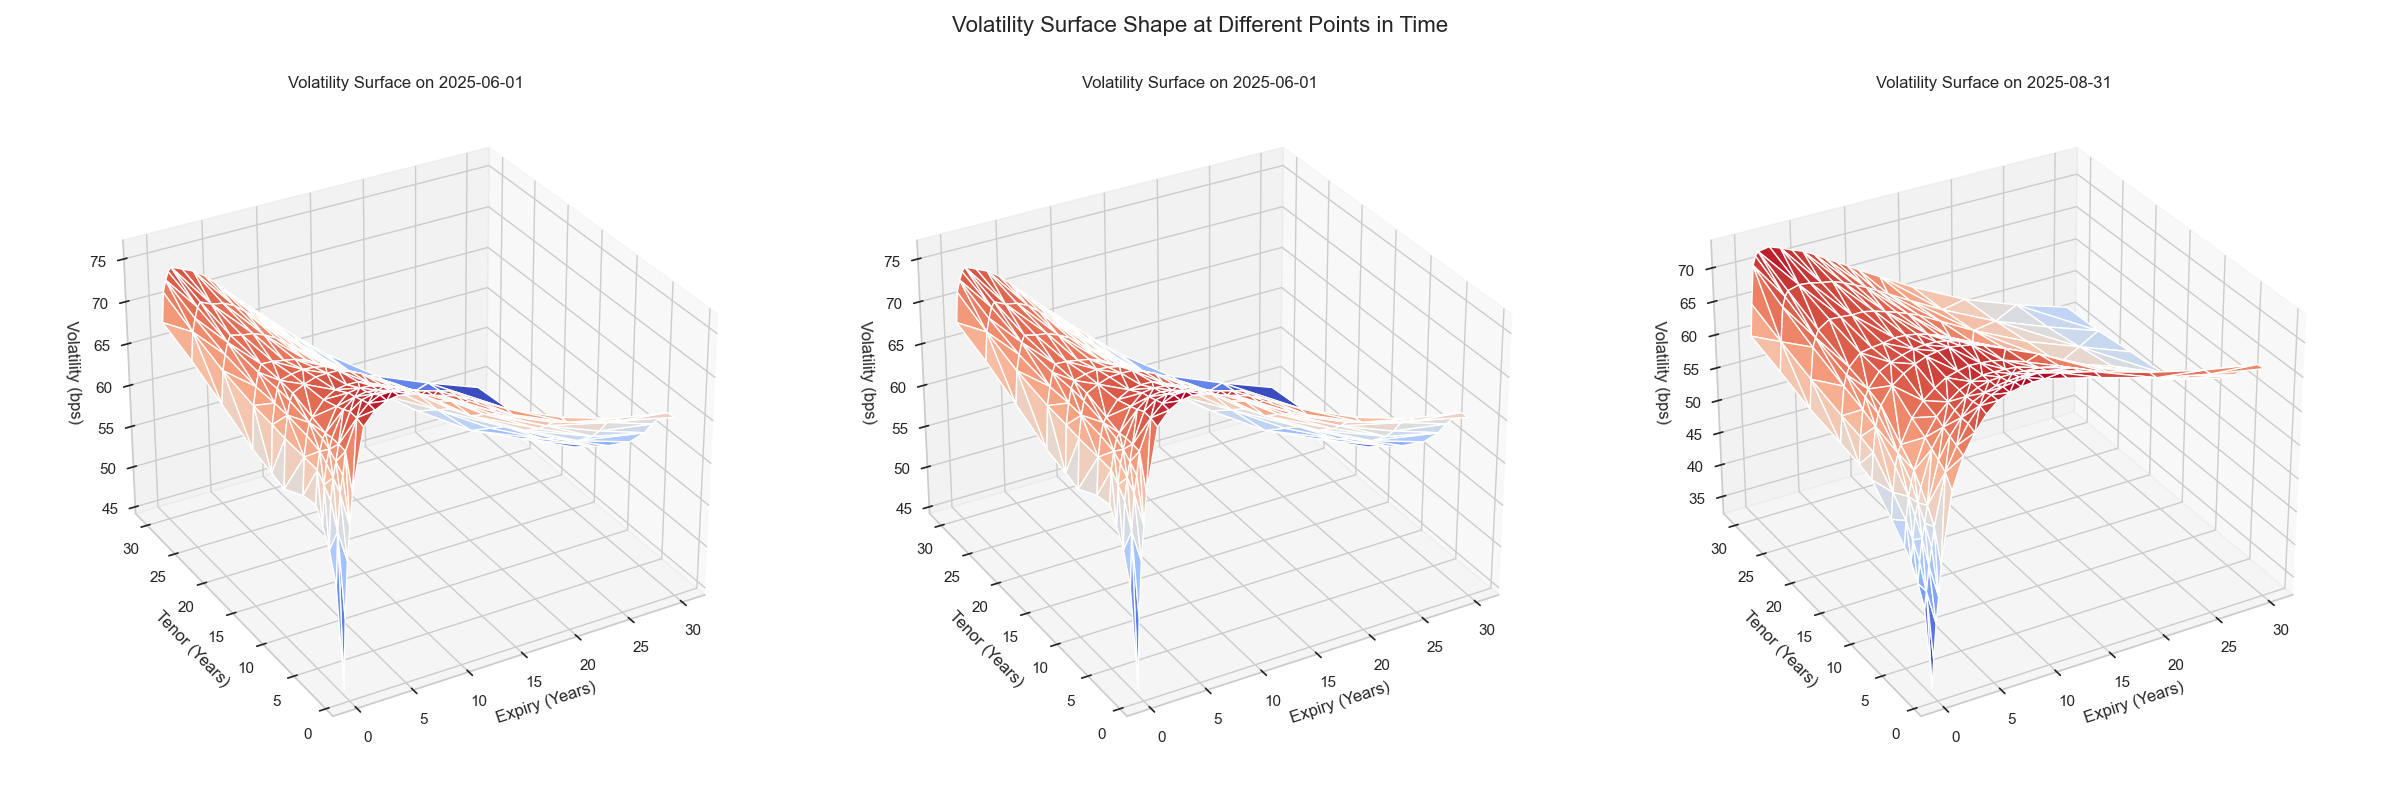
\includegraphics[width=1\textwidth]{images/descriptive_data_analysis/vol_surface_3d_snapshots.png}
	\caption{3D Representation of the Swaption Volatility Surface}
	\label{fig:vol_surface_3d_snapshots}
\end{figure}

Figure~\ref{fig:vol_surface_3d_snapshots} provides a three-dimensional representation of the swaption volatility surface. The surface exhibits pronounced structure, with the highest volatilities concentrated in short-expiry, short-tenor instruments. Volatility decreases along both the expiry and tenor dimensions, forming a characteristic “hump” at the short end. This structural complexity underscores the necessity of employing non-linear modeling approaches—such as neural networks—to accurately capture the surface’s intricate shape and temporal dynamics.

\begin{figure}[H]
	\centering
	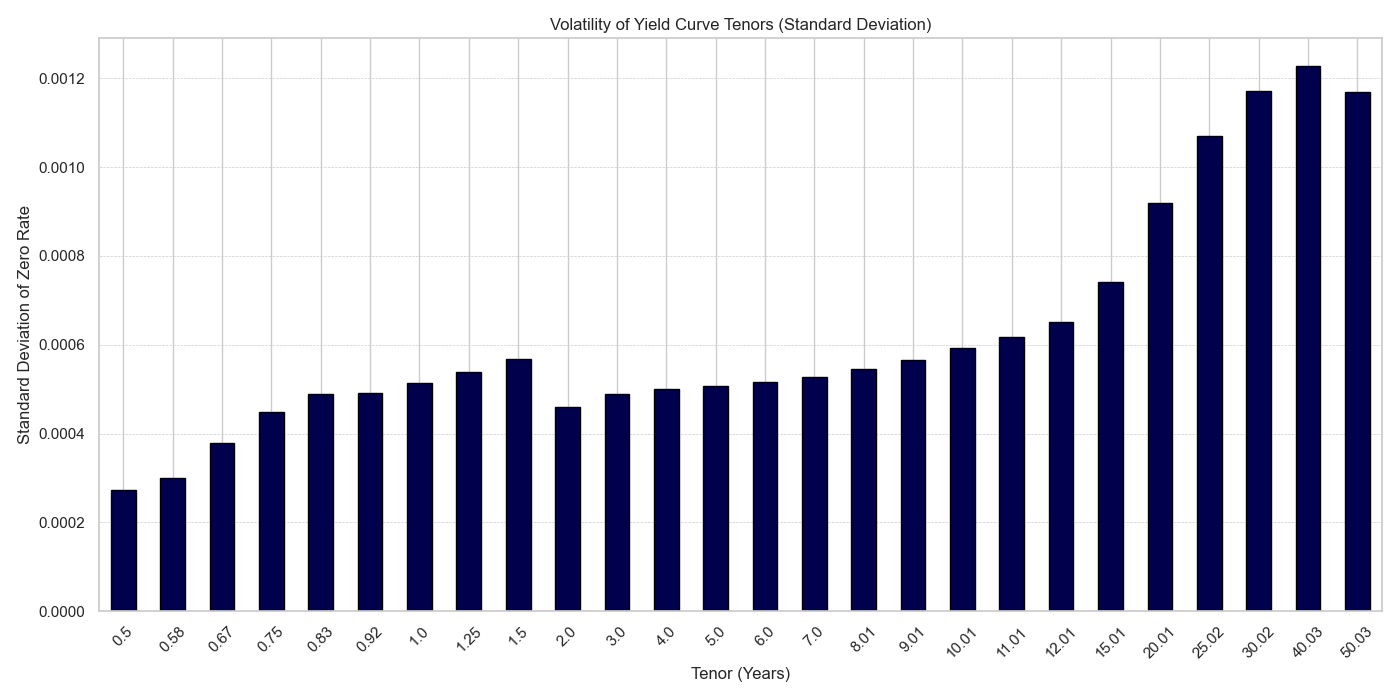
\includegraphics[width=1\textwidth]{images/descriptive_data_analysis/yield_curve_std_by_tenor.png}
	\caption{Standard Deviation of Daily Yield Changes by Tenor}
	\label{fig:yield_curve_std_by_tenor}
\end{figure}

Figure~\ref{fig:yield_curve_std_by_tenor} shows the distribution of yield volatility across maturities. Volatility is lowest at the short end, increases moderately in the 1–2 year range, and rises significantly for longer maturities beyond 10 years. This pattern highlights that long-term yields exhibit the greatest absolute variability, a crucial consideration for risk management and model calibration.

\begin{figure}[H]
	\centering
	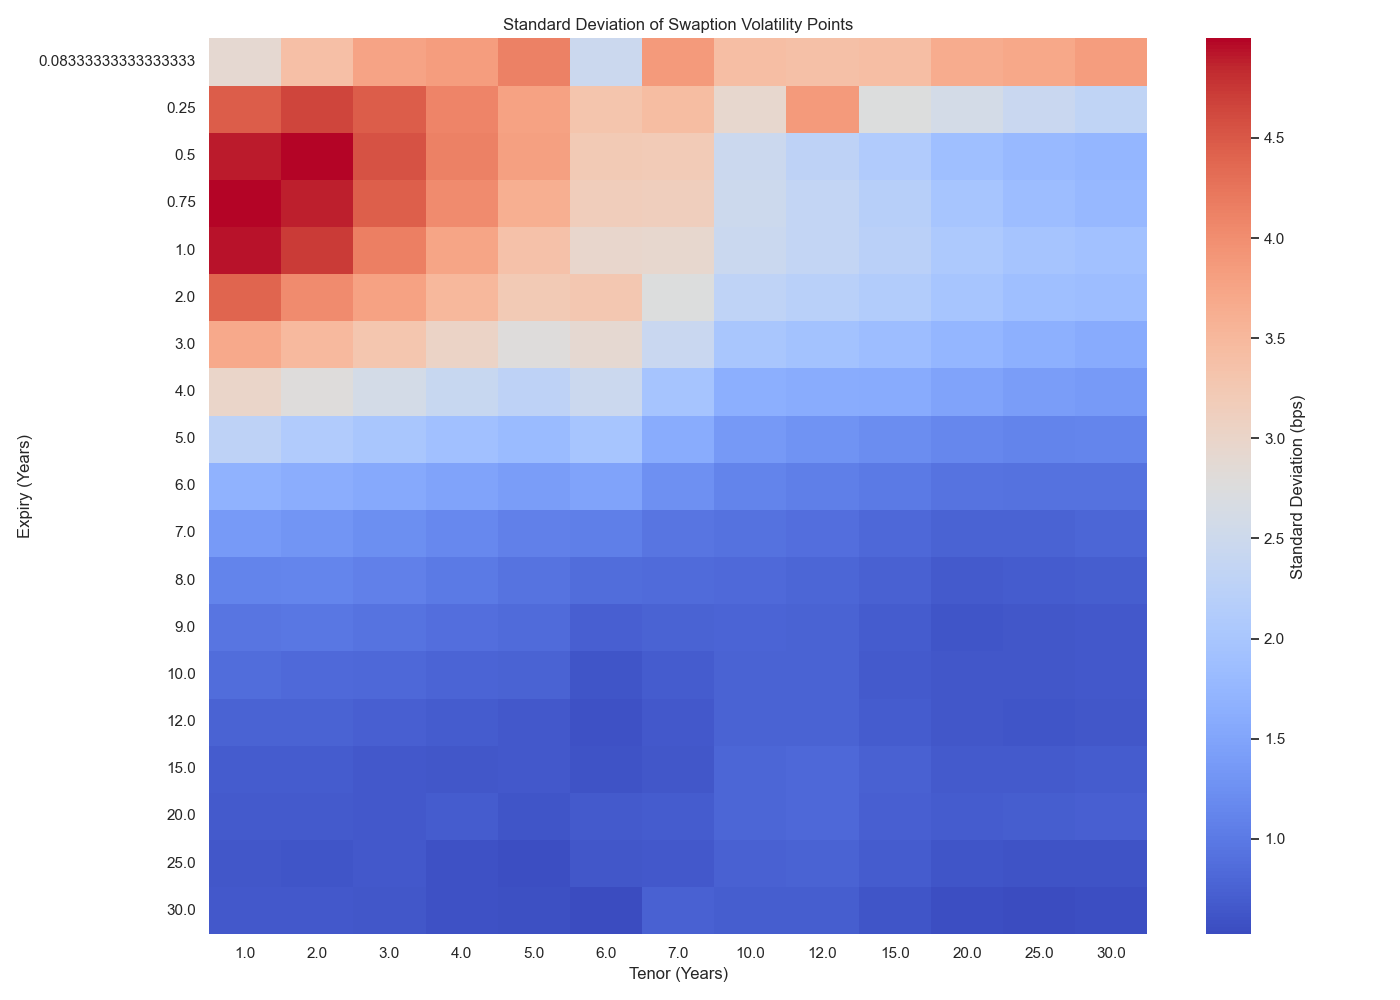
\includegraphics[width=1\textwidth]{images/descriptive_data_analysis/vol_surface_std_heatmap.png}
	\caption{Heatmap of Swaption Volatility Surface Standard Deviations}
	\label{fig:vol_surface_std_heatmap}
\end{figure}

Figure~\ref{fig:vol_surface_std_heatmap} displays the standard deviation of swaption volatilities across expiry and tenor dimensions. The highest volatility—represented by the most intense red shading—is concentrated in the short-expiry, short-tenor region. This indicates that the front end of the surface is particularly unstable, while the long end remains relatively static. A well-performing model must therefore excel at capturing the pronounced temporal variability in this region.

% --- TABLE 3 INSERTED HERE ---
\begin{table}[H]
	\centering
	\begin{threeparttable}
		\caption{Standard Deviation of Swaption Volatilities (in basis points)}
		\label{tab:vol_std_summary}
		\begin{tabular}{lcccc}
			\toprule
			\textbf{Expiry} & \textbf{1-Year Tenor} & \textbf{5-Year Tenor} & \textbf{10-Year Tenor} & \textbf{30-Year Tenor} \\
			\midrule
			1-Year          & 4.93                  & 3.37                  & 2.45                   & 1.92                   \\
			5-Year          & 2.28                  & 1.82                  & 1.35                   & 1.12                   \\
			10-Year         & 0.86                  & 0.75                  & 0.76                   & 0.65                   \\
			30-Year         & 0.66                  & 0.56                  & 0.71                   & 0.54                   \\
			\bottomrule
		\end{tabular}
		\begin{tablenotes}
			\footnotesize
			\item  Standard deviation of daily swaption volatilities, measured in basis points (bps). The table shows the absolute volatility for key points on the expiry-tenor grid.
		\end{tablenotes}
	\end{threeparttable}
\end{table}


Table~\ref{tab:vol_std_summary} provides a quantitative counterpart to the heatmap in Figure~\ref{fig:vol_surface_std_heatmap}, detailing the magnitude of instability across the volatility surface. The data confirms that the highest volatility is located at the front end, with the 1-year expiry, 1-year tenor swaption exhibiting a standard deviation of 4.93 bps. This value is nearly an order of magnitude larger than the 0.54 bps standard deviation observed for the 30-year expiry, 30-year tenor swaption. This sharp gradient in instability underscores the modeling challenge: the neural network must learn to produce highly dynamic outputs for the front end of the surface while generating stable outputs for the back end.

\begin{figure}[H]
	\centering
	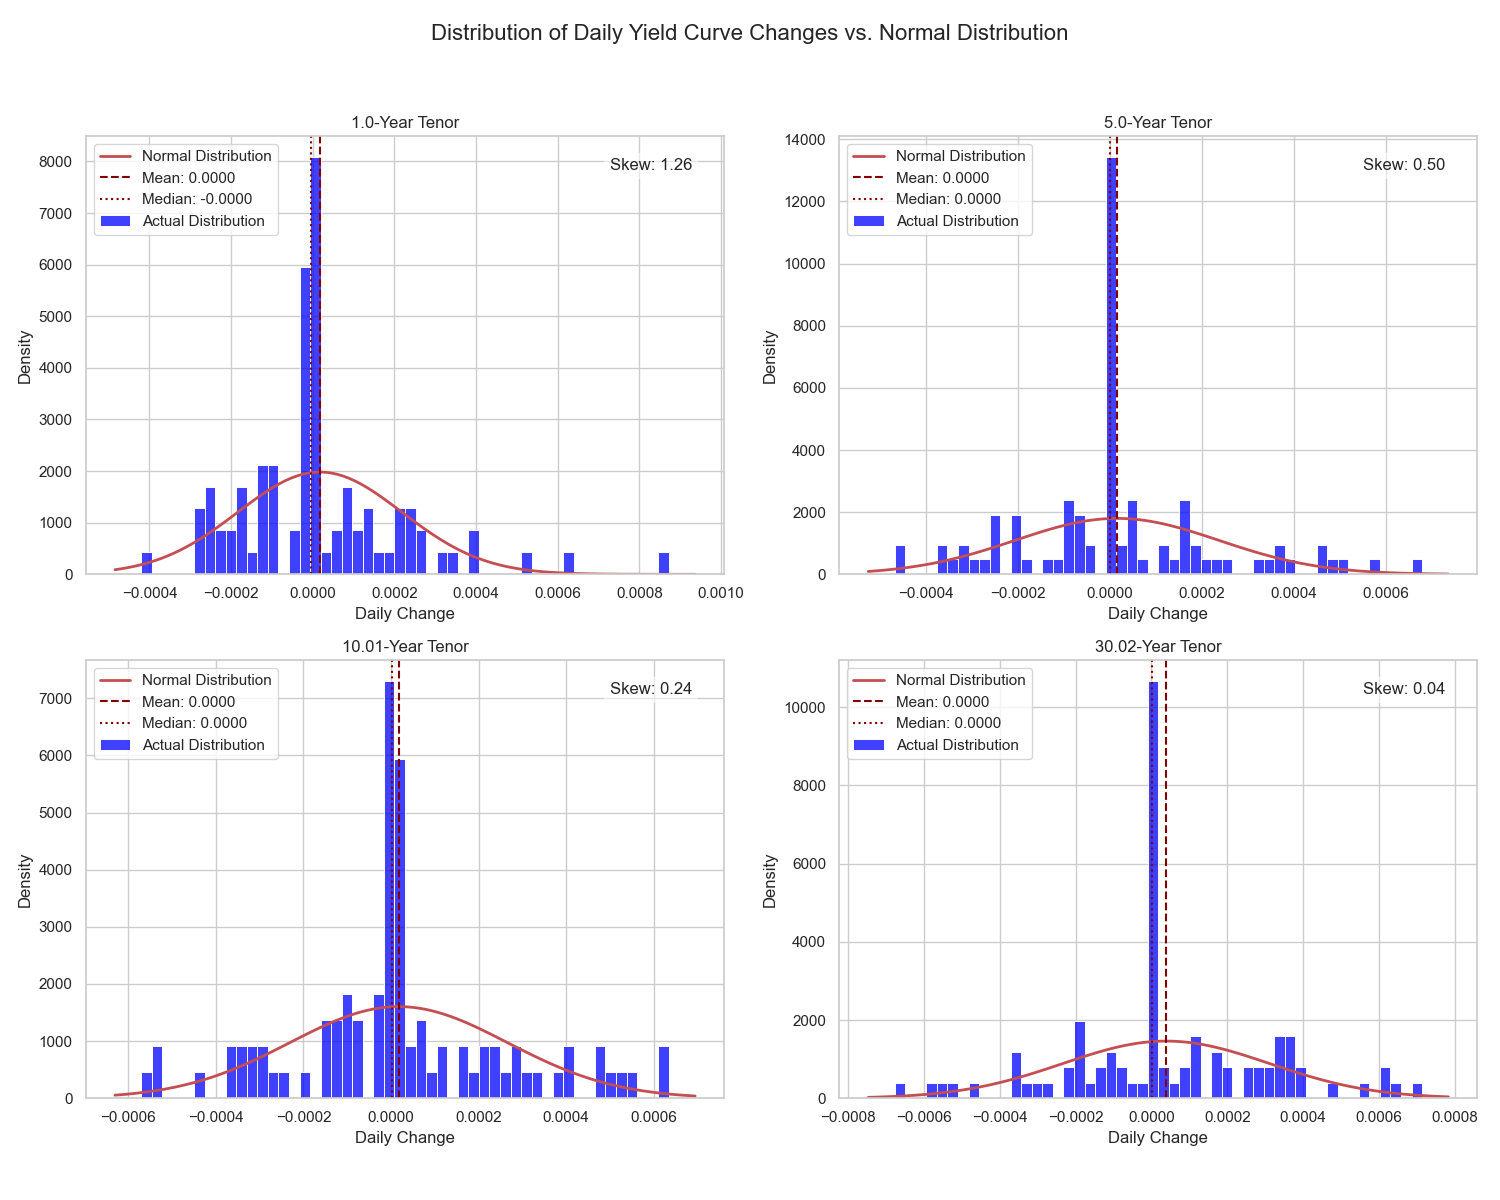
\includegraphics[width=1\textwidth]{images/descriptive_data_analysis/yield_curve_daily_changes_histogram.png}
	\caption{Histograms of Daily Yield Changes by Tenor}
	\label{fig:yield_curve_daily_changes_histogram}
\end{figure}

Figure~\ref{fig:yield_curve_daily_changes_histogram} compares empirical histograms of daily interest rate changes with theoretical normal distributions. All tenors display leptokurtic distributions with fat tails, implying that extreme movements occur more frequently than predicted by Gaussian models. The 1-year tenor exhibits pronounced positive skewness (1.26), suggesting a tendency toward larger upward rate movements. Skewness gradually declines for longer maturities. These findings confirm that interest rate changes deviate substantially from normality.

\begin{figure}[H]
	\centering
	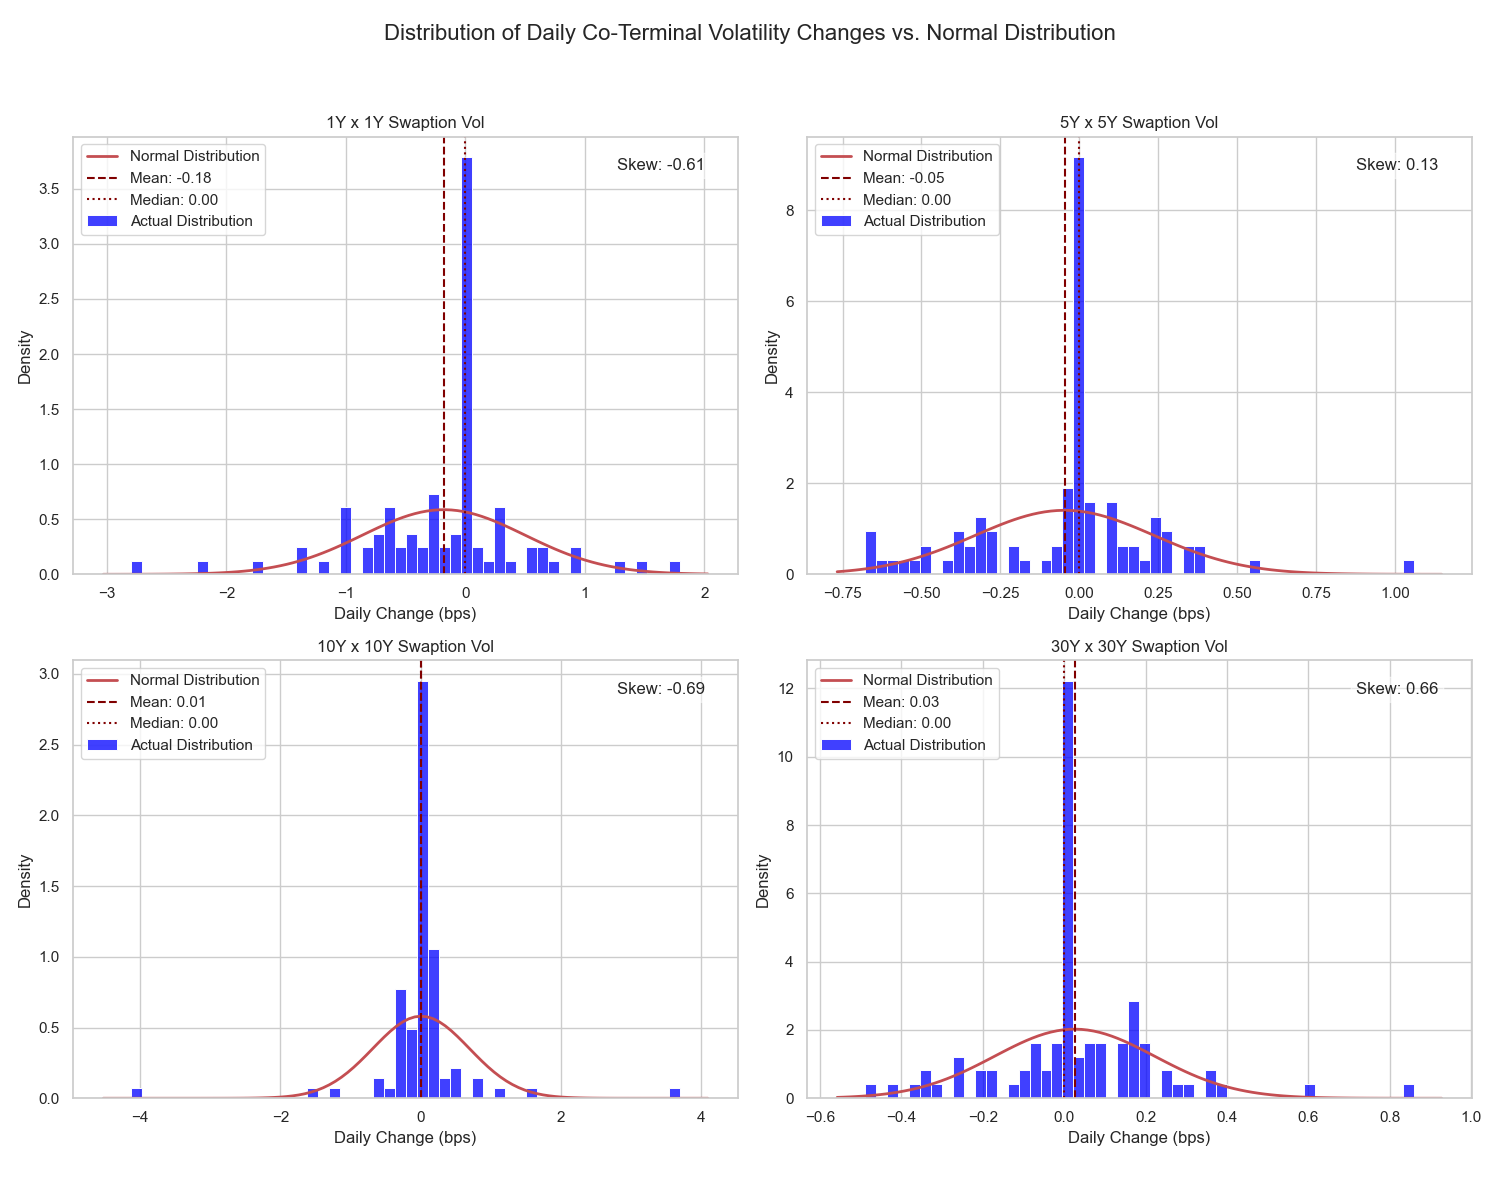
\includegraphics[width=1\textwidth]{images/descriptive_data_analysis/vol_surface_daily_changes_histogram.png}
	\caption{Histograms of Daily Swaption Volatility Changes}
	\label{fig:vol_surface_daily_changes_histogram}
\end{figure}

Figure~\ref{fig:vol_surface_daily_changes_histogram} presents the distribution of daily changes in swaption volatilities. Similar to yield changes, the data exhibit significant leptokurtosis and fat tails, confirming the non-normal nature of the underlying process. A mild positive skew is particularly evident in the 5-year tenor (skew = 0.50), indicating that large volatility spikes are more frequent than declines. Together with the findings from Figure~\ref{fig:yield_curve_daily_changes_histogram}, this evidence supports the use of non-parametric, data-driven models—such as neural networks—that can flexibly capture these empirical deviations from normality.

\subsection{Data Preprocessing}
\subsubsection{Bootstrapping Zero-Curves}
The implementation of the one-factor Hull–White model in \texttt{QuantLib} requires zero-coupon curves as input for both discounting and forward-rate generation. Consequently, the EUR swap curves obtained from Bloomberg were bootstrapped into continuous zero-rate term structures following the procedure outlined in subsection~\ref{subsec:bootstrap_zero_curve}. This ensures compatibility with the \texttt{QuantLib} framework and provides a consistent foundation for pricing swaptions and calibrating the model parameters.

\subsubsection{Handling Non-Trading Days in External Data}
The external market data obtained from Yahoo Finance, including the MOVE index, VIX index, and EUR/USD exchange rate, is only available for trading days. In contrast, the swaption and swap curve datasets contain values for all calendar days, including weekends and public holidays. To ensure temporal consistency across all features used for Hull–White model calibration, the external data were reindexed to cover the entire daily date range of the analysis period.

Missing values corresponding to non-trading days were filled using a combination of forward-filling and {backward-filling. Forward-filling propagates the most recent available value to subsequent missing days, while backward-filling assigns the nearest subsequent available value to preceding missing days. This procedure ensures that every day within the observation window has a corresponding value for each external variable, resulting in a continuous dataset that can be used by the neural network without introducing gaps or inconsistencies.

\subsubsection{Feature Engineering for the Neural Network}
In addition to the raw market data, several engineered features were created to enhance the neural network's ability to predict Hull–White model parameters. These features capture the shape of the yield curve, relationships between external market indicators, and underlying latent structures via dimensionality reduction. Each feature was designed with a clear economic or statistical justification for its relevance to the model parameters: the volatility \(\sigma\) and the mean-reversion speed \(a\).

\paragraph{Features Engineered from the Yield Curve}
These features explicitly describe the shape and dynamics of the zero-coupon interest rate term structure. Let \(\text{Rate}(T)\) denote the zero-coupon rate for a given tenor \(T\) (e.g., \(\text{Rate}(10\text{Y})\) is the 10-year rate).

\textit{Slope Features:}
\begin{equation}
	\text{slope\_3m10y} = \text{Rate}(10\text{Y}) - \text{Rate}(3\text{M})
\end{equation}

\begin{equation}
	\text{slope\_2y10y} = \text{Rate}(10\text{Y}) - \text{Rate}(2\text{Y})
\end{equation}

\begin{equation}
	\text{slope\_5y30y} = \text{Rate}(30\text{Y}) - \text{Rate}(5\text{Y})
\end{equation}

A steep positive slope typically signals expectations of economic growth and future rate hikes, implying higher expected interest rate volatility (\(\sigma\)). Conversely, a flat or inverted curve suggests a more stable rate environment and lower \(\sigma\). Regarding mean reversion (\(a\)), a steep curve indicates strong anchoring to the long-term average, implying higher \(a\), while an inverted curve signals weaker anchoring and lower \(a\).

\textit{Curvature Features:}
\begin{equation}
	\text{curvature\_2y5y10y} = 2 \cdot \text{Rate}(5\text{Y}) - \text{Rate}(2\text{Y}) - \text{Rate}(10\text{Y})
\end{equation}

\begin{equation}
	\text{curvature\_1y2y5y} = 2 \cdot \text{Rate}(2\text{Y}) - \text{Rate}(1\text{Y}) - \text{Rate}(5\text{Y})
\end{equation}

\begin{equation}
	\text{curvature\_10y20y30y} = 2 \cdot \text{Rate}(20\text{Y}) - \text{Rate}(10\text{Y}) - \text{Rate}(30\text{Y})
\end{equation}

High curvature indicates significant uncertainty in medium-term rates, aiding prediction of the term structure of \(\sigma\). Pronounced curvature suggests rates are expected to revert to a mean, implying higher \(a\). Flat curvature indicates weaker mean reversion and lower \(a\).

\paragraph{Features Engineered from External Market Data} \mbox{}\\
\textit{Curvature-to-Slope Ratio:}
\begin{equation}
	\text{curvature\_slope\_ratio} = \frac{\text{curvature\_2y5y10y}}{\text{slope\_2y10y}}
\end{equation}
This feature captures nuanced market regimes where slope and curvature provide complementary information. It allows the network to distinguish between different economic environments and predict both \(\sigma\) and \(a\) more accurately.

\textit{MOVE-to-VIX Ratio:}
\begin{equation}
	\text{MOVE\_VIX\_Ratio} = \frac{\text{MOVE\_Open}}{\text{VIX\_Open}}
\end{equation}
A high ratio indicates stress concentrated in the bond market, signaling a higher \(\sigma\) specific to interest rates. It also implies uncertainty about central bank policy, potentially reducing \(a\). This feature helps the network separate general market panics from fixed-income-specific volatility.

\paragraph{Features Engineered via Dimensionality Reduction}
Instead of feeding all individual zero-coupon rates directly into the neural network, the yield curve was transformed using Principal Component Analysis (PCA). The reason for this choice lies in the fact that individual rates on the curve are highly correlated — a move in the 5-year rate is almost always accompanied by similar movements in the 7-year and 10-year rates as visible in figure \ref{fig:feature_correlation_prePCA}. Using these raw, correlated rates introduces several problems: multicollinearity, redundant information, and an increased risk of overfitting.

\begin{figure}[H]
	\centering
	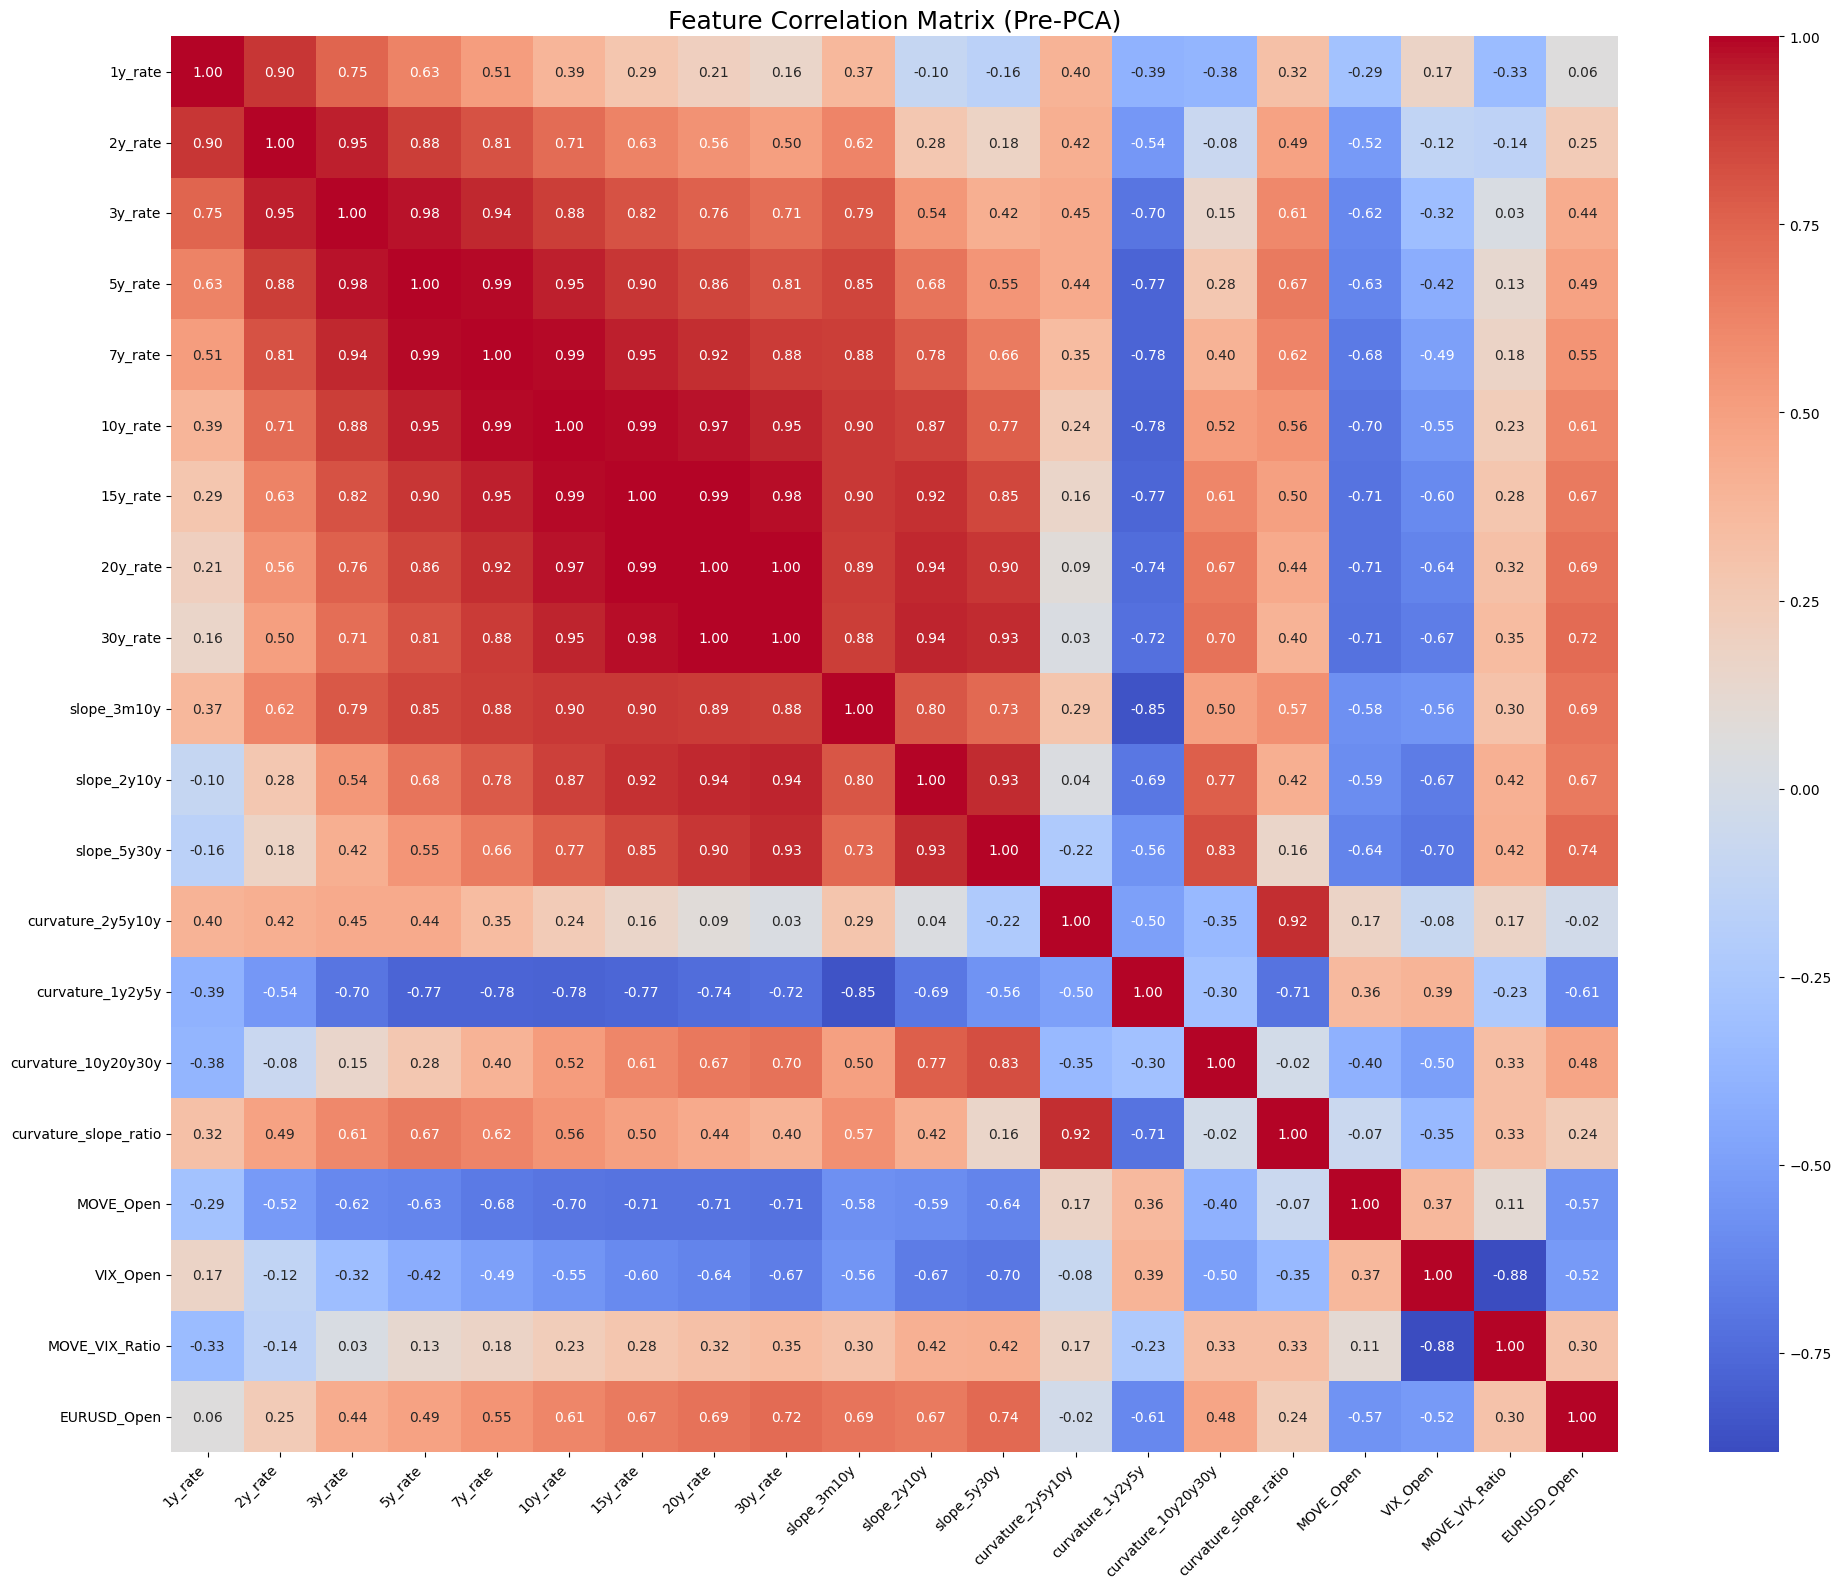
\includegraphics[width=1\textwidth]{images/features/feature_correlation_matrixPre-PCA.png}
	\caption{Correlation matrix of the engineered features before applying PCA.}
	\label{fig:feature_correlation_prePCA}
\end{figure}

Multicollinearity causes instability in the learned weights of the neural network. When input features contain overlapping information, the model struggles to assign stable importance to each feature. It may assign large, offsetting weights to features that move together, resulting in unstable and unreliable predictions \parencite[p.~2]{chan2022multicollinearity}.

Redundant information makes the learning process inefficient and typically leads to poor test performance \parencite[p.~3]{sildir2020redudantfeatures}. Most daily movements in the yield curve are dominated by a single pattern — a parallel shift. Feeding the model all the raw rates forces it to re-learn this shared structure repeatedly instead of focusing on economically meaningful dynamics such as slope or curvature changes.

High dimensionality further increases the complexity of the model, encouraging overfitting. With too many correlated features, the neural network risks memorizing noise instead of generalizable relationships, which harms out-of-sample performance \parencite[p.~3]{sildir2020redudantfeatures}.

PCA directly resolves these issues by transforming the vector of rates
\[
	R = [\text{Rate}(1\text{Y}), \text{Rate}(2\text{Y}), \dots, \text{Rate}(30\text{Y})]
\]
into a set of uncorrelated and economically interpretable components:
\begin{equation}
	\text{PC\_Level} = \mathbf{w}_1 \cdot \mathbf{R}
\end{equation}
\begin{equation}
	\text{PC\_Slope} = \mathbf{w}_2 \cdot \mathbf{R}
\end{equation}
\begin{equation}
	\text{PC\_Curvature} = \mathbf{w}_3 \cdot \mathbf{R}
\end{equation}

These three “super-features” capture nearly all the meaningful variation of the yield curve and can be interpreted as follows \parencite[pp.~98--107]{Rebonato_2018}:
\begin{itemize}
	\item PC\_Level represents the overall interest rate level and captures parallel shifts. Empirically, higher rate levels are associated with higher volatility (\(\sigma\)).
	\item PC\_Slope measures the steepness of the curve and reflects economic expectations, influencing both \(\sigma\) and \(a\).
	\item PC\_Curvature captures the non-linear “bow” of the curve, aiding the model in learning term-structure effects in the piecewise $\sigma$ and mean-reversion dynamics $\alpha$.
\end{itemize}

After applying PCA to the engineered features, the resulting correlation matrix exhibits a significant reduction in the highest correlations. The originally strong dependencies between individual yield curve rates and other features are largely removed as visible in figure \ref{fig:feature_correlation_postPCA}, demonstrating that the principal components provide a set of largely uncorrelated, independent features for the neural network.

\begin{figure}[H]
	\centering
	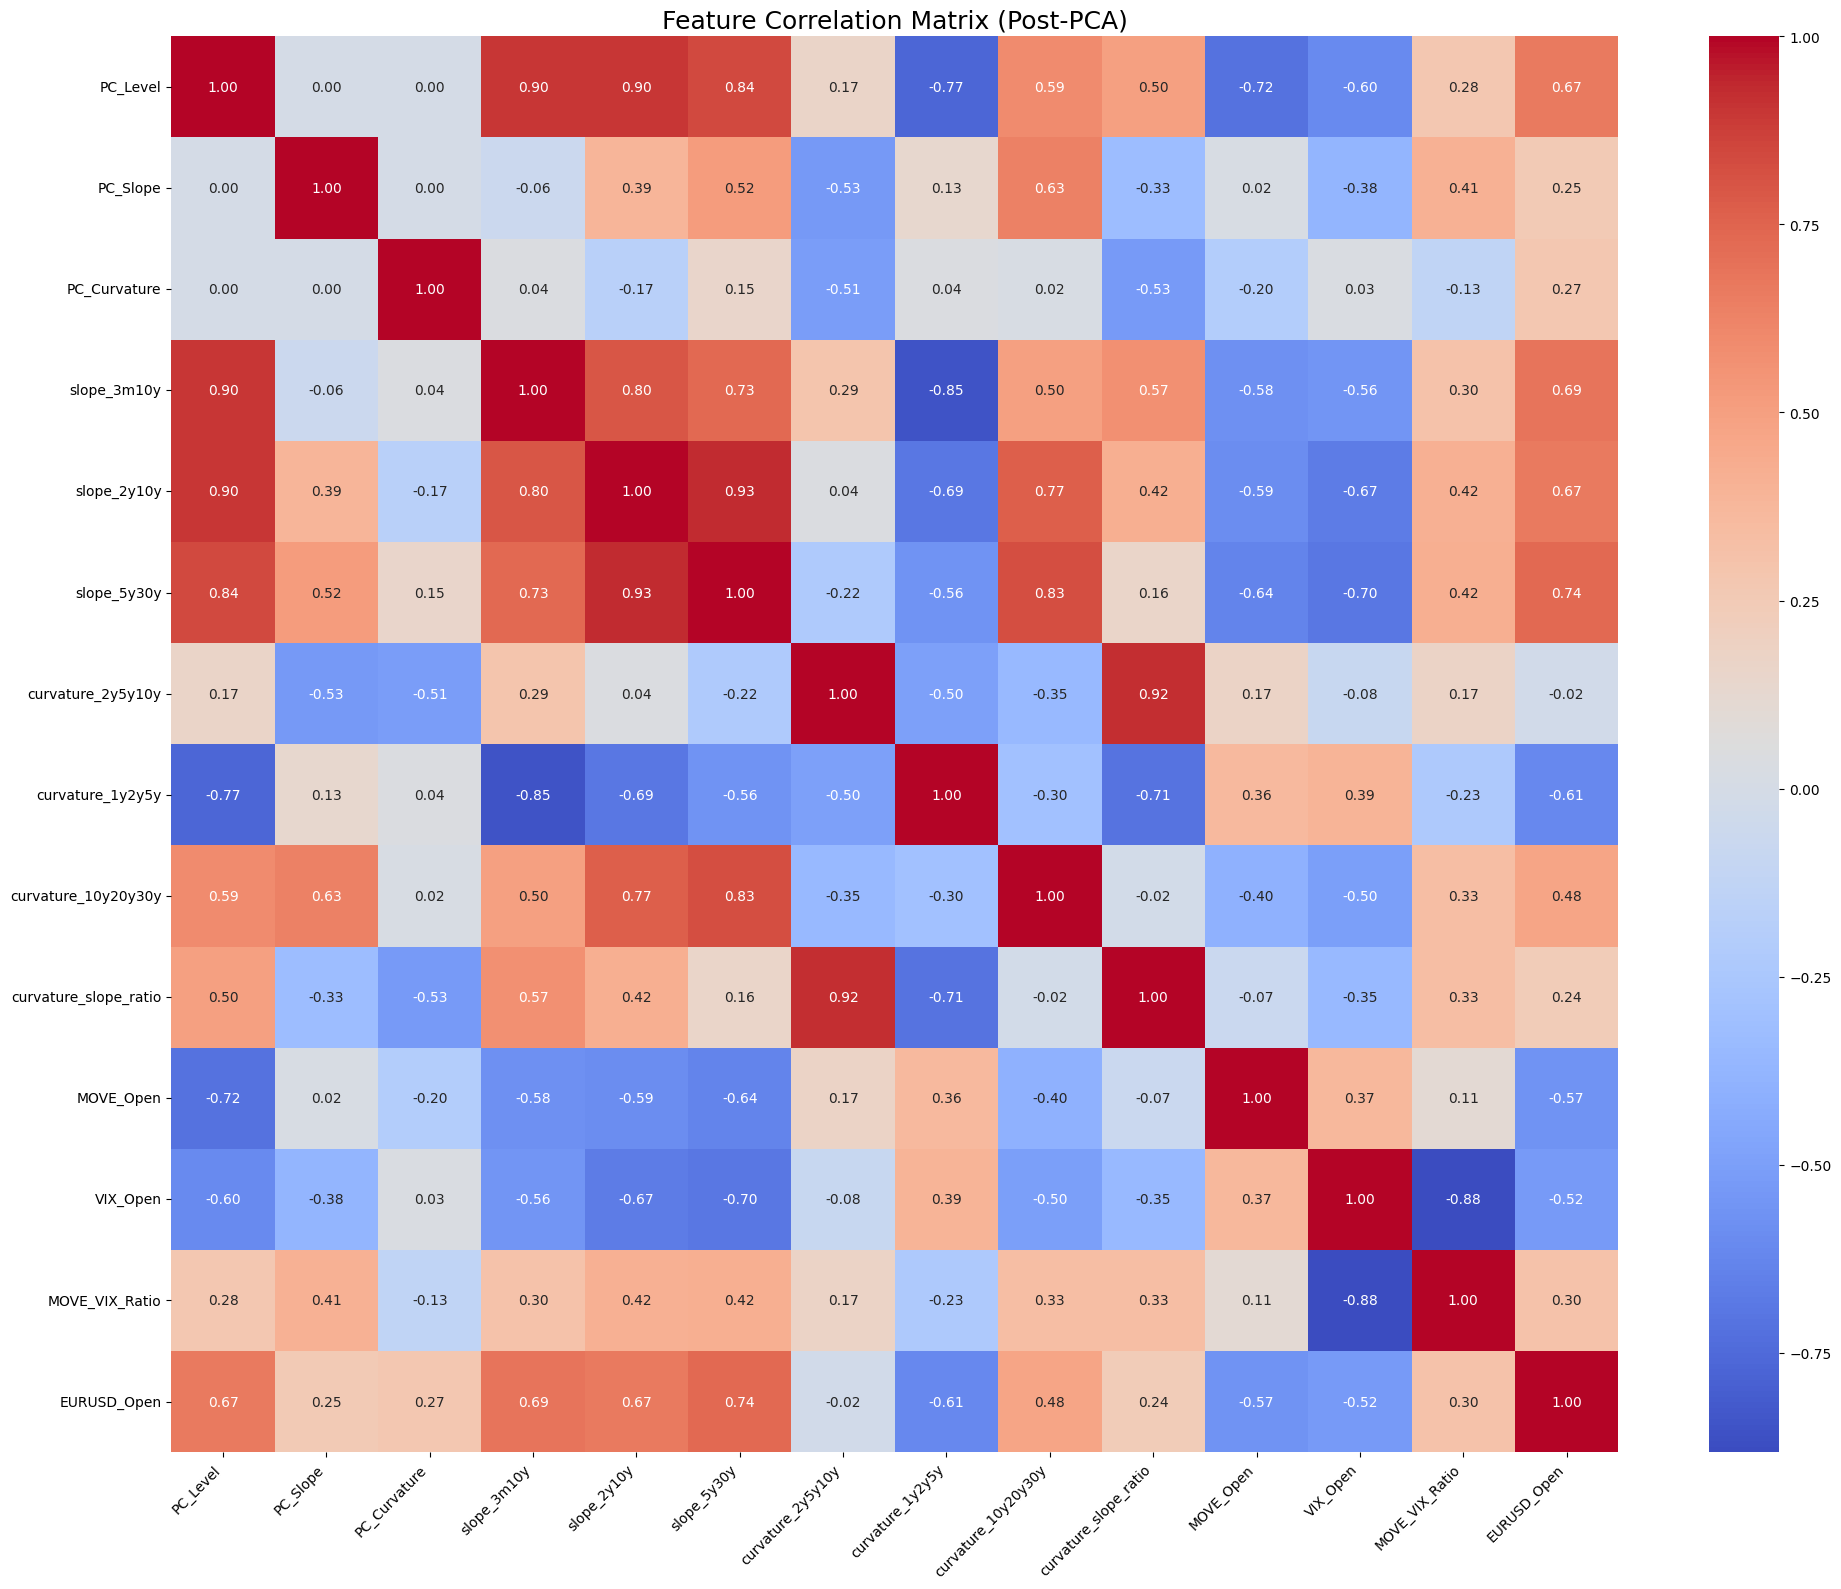
\includegraphics[width=1\textwidth]{images/features/feature_correlation_matrixPost-PCA.png}
	\caption{Correlation matrix of the engineered features after applying PCA.}
	\label{fig:feature_correlation_postPCA}
\end{figure}

By reducing the dimensionality from roughly ten correlated rate inputs to three independent components, PCA provides a stable, interpretable, and compact representation of the yield curve. This significantly improves the neural network’s training efficiency, robustness, and generalization performance.

\subsubsection{Feature Scaling}
Prior to being fed into the neural network, all input features are scaled using the \texttt{StandardScaler} from the \texttt{scikit-learn} library. This process, also known as standardization or Z-score normalization, ensures that each feature has a mean of zero and a standard deviation of one \parencite[pp.~31--32]{zheng2018feature}.

The scaling process consists of two main steps:

\textit{Step 1: Fit Phase (Learning from Training Data)}
The scaler analyzes the training data to learn the distribution of each feature. For each feature column, it calculates:

\begin{equation}
	\mu = \frac{1}{n} \sum_{i=1}^{n} x_i
\end{equation}
\begin{equation}
	\sigma = \sqrt{\frac{1}{n} \sum_{i=1}^{n} (x_i - \mu)^2}
\end{equation}

where \(x_i\) are the individual values of the feature and \(n\) is the number of training samples. The computed mean \(\mu\) and standard deviation \(\sigma\) are stored in the scaler object.

\textit{Step 2: Transform Phase (Applying the Scaling)}
The learned parameters are used to transform all values of that feature in the training, validation, and test datasets:

\begin{equation}
	z = \frac{x - \mu}{\sigma}
\end{equation}

This centers the data around zero and scales it to unit variance.

From a computational perspective, normalization is necessary to manage issues arising from the inherent structure of raw data inputs. It is a technique widely used in statistics for making the units of variables comparable, which is critical when input data are expressed in very different units and exhibit disparate orders of magnitude. Without scaling, features with very large numerical values can dominate the error calculation, causing the error reduction algorithm to focus primarily on these variables while neglecting the information contained in smaller-valued features. Furthermore, when raw numerical values are extremely large, such as on the order of $10^{6}$, their processing can generate outputs that exceed the capacity of standard computing hardware, making scaling essential to control for calculation and roundoff errors \parencite{shanker1996effectdatastandardization}.

The application of scaling directly addresses the optimization landscape of the training problem, leading to more efficient convergence. Normalizing the input is known to accelerate convergence during the optimization of linear models. Linear scale transformations, especially those that compress the search space, reduce the distance the backpropagation algorithm must cover in each iteration \parencite{sola1997importancedatanormalization}. This improved conditioning, where normalization helps ensure the covariance matrix of the layer input $\sum{}x$ is well-conditioned, is crucial for faster learning and aids the optimization algorithm in locating local minima \parencite{huang2020normalizationtechniquestrainingdnns}. Consequently, an adequate normalization protocol can significantly reduce calculation and training time, with studies showing that estimation errors can be reduced by a factor of 5 to 10 and the time required to achieve such results reduced by an order of magnitude \parencite{sola1997importancedatanormalization}.

Ultimately, the primary result of standardization is an improvement in the neural network's quality and training stability. Data transformation is frequently used for improved learning, and normalization techniques are considered essential for accelerating the training and enhancing the generalization of deep neural networks (DNNs). Networks trained on standardized data generally yield better overall results, leading to a higher classification rate and a smaller Mean Square Error (MSE) in regression problems, where a smaller MSE indicates a higher quality solution \parencite{shanker1996effectdatastandardization}. The performance of a network, including the number of training iterations required and the final error attained, is enhanced as the input variable ranges are 'equalized' by the normalization process. This contributes to scale-invariant learning, which is important for stabilizing training and has been shown to be useful for adaptively adjusting the learning rate. In some cases, standardization is not merely a best practice but a formal prerequisite due to specific algorithm requirements \parencite{huang2020normalizationtechniquestrainingdnns}.

By applying \texttt{StandardScaler}, the neural network receives a well-conditioned, standardized input, which improves training stability, and convergence speed of the resulting model.

\subsection{Hyperparameter Optimization}
\label{subsec:hyperparameter_optimization}

The predictive performance and stability of neural networks depend critically on an appropriate choice of hyperparameters. To identify an optimal configuration, a structured hyperparameter optimization process was conducted using the Hyperband algorithm, as described in Subsection~\ref{subsec:hyperband_algorithm}. This algorithm efficiently allocates computational resources to explore a broad hyperparameter space while focusing on the most promising configurations.

The core settings for the Hyperband tuner were configured as follows:
\begin{itemize}
	\item Maximum Epochs per Trial (\texttt{max\_epochs}): A total of 1000 epochs were allocated as the maximum budget for training any single hyperparameter configuration.
	\item Reduction Factor (\texttt{factor}): A factor of 3 was used, meaning that after each round of training within a bracket, the number of configurations is reduced by a factor of 3, retaining only the top-performing third.
	\item Objective: The optimization objective was the minimization of the root mean squared error on the validation set.
\end{itemize}

The hyperparameters tuned in this study can be divided into two categories: those defining the neural network architecture and those related to the training process and loss function. Hyperparameters related to the architecture are:
\begin{itemize}
	\item Number of Hidden Layers: This parameter determines the depth of the neural network. A deeper network has greater representational power and can capture more complex nonlinear relationships in the data, but it also increases the risk of overfitting and computational cost. \newline
	      \textit{Search Space:} Integer between 1 and 5
	\item Number of Neurons per Layer: The width of each hidden layer, determined by the number of neurons, controls the capacity of the model. Larger layers allow for more detailed pattern recognition but can lead to overfitting if excessive. \newline
	      \textit{Search Space:} Integer between 16 and 128, in steps of 16, for each hidden layer
	\item The activation function introduces non-linearity into the network, enabling it to model complex relationships between input features and outputs. \newline
	      \textit{Search Space:} Choice between \texttt{relu} and \texttt{tanh}.
	\item Dropout is a regularization technique that randomly deactivates a fraction of neurons during training to prevent overfitting by discouraging co-adaptation among neurons. \newline
	      \textit{Search Space:} Boolean choice between \texttt{True} and \texttt{False}.
	\item Dropout Rate: If dropout is used, this parameter determines the fraction of neurons dropped during each training iteration. \newline
	      \textit{Search Space:} Floating-point value between 0.1 and 0.5 (only active if \texttt{use\_dropout = True}) in steps of 0.1.

\end{itemize}

Tuneable hyperparameters which cover the training and the loss functions are:
\begin{itemize}
	\item Learning Rate: The learning rate governs the step size used by the optimizer when updating the model’s weights. A high learning rate may lead to instability or divergence, whereas a very low one results in slow convergence. To capture effective values across orders of magnitude, the search was conducted on a logarithmic scale. \newline
	      \textit{Search Space:} Floating-point value between 0.0001 and 0.01, sampled logarithmically.

	\item Underestimation Penalty: This custom hyperparameter is designed to address the asymmetric cost of forecasting errors in financial volatility modeling. Underestimating volatility poses a greater financial risk than overestimating it. Therefore, this penalty increases the loss when the model underpredicts volatility, encouraging more conservative estimates. \newline
	      \textit{Search Space:} Floating-point value between 0.5 (penalty for overestimation) and 4.0 (strong penalty) in steps of 0.1.
\end{itemize}

\subsection{Loss Function and Error Metric}

The objective of the neural network is to determine the optimal set of weights W and biases b such that the predicted Hull--White parameters minimize the discrepancy between model-implied swaption volatilities and their market-observed counterparts. The neural network acts as a function
\begin{equation}
	\text{NN} : x \mapsto \theta(x; W, b),
\end{equation}
where $x \in \mathbb{R}^d$ is the input feature vector containing scaled and PCA-transformed market data (yield curve levels, slopes, curvatures, etc.) for a given day, and $\theta$ denotes the vector of Hull--White model parameters to be predicted. The network employs a residual architecture: instead of predicting $\theta$ directly, it predicts a deviation $\Delta z$ from a fixed initial guess $z_0$:
\begin{equation}
	\Delta z = \text{NN}(x; W, b), \quad
	z = z_0 + \Delta z.
\end{equation}
The predicted parameters are obtained by applying a scaled sigmoid to ensure they remain within a predefined range [0, U]:
\begin{equation}
	\theta(x; W, b) = U \cdot \sigma(z) = U \cdot \frac{1}{1 + e^{-z}}.
\end{equation}

The predicted parameters $\theta$ are subsequently used within the QuantLib library as a black-box function $V_{\text{QL}}$, which computes model-implied volatilities $\hat{\sigma}$ for a portfolio of $n$ swaptions given the additional market data $M_j$ on day $j$:
\begin{equation}
	\hat{\sigma} = V_{\text{QL}}(\theta, M_j) = \{\hat{\sigma}_1, \hat{\sigma}_2, \dots, \hat{\sigma}_n\}.
\end{equation}

The predictive accuracy of the network is quantified using the root mean squared error (RMSE), which measures the average magnitude of deviation between model-implied and market-observed volatilities, expressed in basis points (bps):
\begin{equation}
	\text{RMSE} = \sqrt{\frac{1}{n}\sum_{i=1}^{n}(\hat{\sigma}_i - \sigma_i)^2} \times 10000.
\end{equation}

\begin{table}[H]
	\centering
	\caption{Notation used in the RMSE formula}
	\begin{tabular}{lp{12cm}}
		\toprule
		Symbol  & Meaning                                                                                                                   \\
		\midrule
		$n$              & Total number of swaptions in the evaluation dataset                                                                                \\
		$\hat{\sigma}_i$ & Implied volatility predicted by the Hull--White model using the parameters generated by the neural network for the $i$-th swaption \\
		$\sigma_i$       & Market-observed implied volatility for the $i$-th swaption                                                                         \\
		\bottomrule
	\end{tabular}
\end{table}

To align the optimization with practical calibration objectives, an asymmetric loss function is employed during training. For each day $j$, the loss is computed as the mean of weighted squared errors between predicted and observed volatilities:
\begin{equation}
	L_j(W, b) = \frac{1}{n} \sum_{i=1}^{n} w_i (\hat{\sigma}_i - \sigma_{j,i})^2,
\end{equation}
where the weight $w_i$ accounts for underestimation penalties:
\begin{equation}
	w_i =
	\begin{cases}
		P, & \text{if } \hat{\sigma}_i < \sigma_{j,i} \quad \text{(underestimation)},   \\
		1, & \text{if } \hat{\sigma}_i \geq \sigma_{j,i} \quad \text{(overestimation)}.
	\end{cases}
\end{equation}
Here, $P>1$ is the underestimation penalty, treated as a hyperparameter optimized using the Hyperband algorithm. This asymmetric weighting is applied exclusively during training to encourage conservative predictions, while evaluation on validation and test sets uses the standard (unweighted) RMSE to assess predictive accuracy objectively.

The overall training objective is to identify network parameters $(W^*, b^*)$ that minimize the expected daily loss over the distribution of training data $D$:
\begin{equation}
	(W^*, b^*) = \arg \min_{W, b} \ \mathbb{E}_{(x_j, \sigma_j, M_j) \sim D} \left[ L_j(W, b) \right].
\end{equation}
In practice, this expectation is approximated by iterating over the training set day by day (batches) using the stochastic optimizer Adam:
\begin{equation}
	W_{t+1} = W_t - \eta \nabla_W L_j(W_t, b_t),
\end{equation}
where $\eta$ is the learning rate. Since $V_{\text{QL}}$ is a non-differentiable black-box function, gradients are computed numerically via finite differences using a tf.custom\_gradient implementation.

\subsection{Methodology Workflow}
The subsequent section delineates the comprehensive, step-by-step workflow implemented for the calibration of the Hull-White model, as depicted by the provided source code. The process is designed as an end-to-end pipeline, commencing with raw data ingestion and culminating in model evaluation, adaptive retraining, and interpretability analysis.

\begin{enumerate}
	\item \textbf{Data Ingestion and Preprocessing:}
	      The initial phase involves loading raw EUR swap curve data, provided in Excel format. For each historical date, the mid-market rate is computed from the bid and ask quotes. These raw swap curves are then processed and transformed into a standardized format. Subsequently, the \texttt{QuantLib} library is employed to bootstrap these swap curves, yielding the corresponding zero-coupon yield curves for each valuation date. This bootstrapping process utilizes a \texttt{PiecewiseLogLinearDiscount} methodology to construct a term structure of zero rates from the observed market swap rates.

	\item \textbf{External Market Data Integration:}
	      To enrich the feature set, external market data is loaded. This includes the ICE BofA MOVE Index (MOVE), which measures US Treasury rate volatility; the CBOE Volatility Index (VIX), which measures equity market volatility; and the EUR/USD foreign exchange rate. This data is sourced via the \texttt{yfinance} library. A complete time series is ensured by forward- and back-filling any missing daily values, providing a consistent set of external features for every yield curve date.

	\item \textbf{Chronological Data Splitting:}
	      Given the time-series nature of the financial data, a strict chronological split is enforced to prevent look-ahead bias. The dataset of available daily yield curves is divided into a training set (the initial 50\%), a validation set (the following 20\%), and a final out-of-sample testing set (the remaining 30\%). This ensures that the model is trained on past data, validated on more recent data, and finally tested on unseen future data.

	\item \textbf{Feature Engineering and Dimensionality Reduction:}
	      For each yield curve, a comprehensive feature vector is engineered. This vector includes not only the zero rates at key tenors (1Y to 30Y) but also derived features such as various yield curve slopes (e.g., 10Y-2Y), curvatures (e.g., $(2 \times 5\text{Y}) - 2\text{Y} - 10\text{Y}$), and the external market indicators. To address the high multicollinearity inherent in yield curve rates, Principal Component Analysis (PCA) is performed exclusively on the rate-based features of the training data. The first three principal components, which typically correspond to the level, slope, and curvature of the yield curve, are retained. This reduces dimensionality while preserving the most significant sources of variance. The complete feature set, comprising these principal components and the other engineered features, is then standardized using Scikit-learn's \texttt{StandardScaler}, which is also fitted solely on the training data.

	\item \textbf{Hyperparameter Optimization:}
	      A rigorous hyperparameter tuning process is conducted using the Hyperband algorithm, implemented via the \texttt{Keras Tuner} library. The search space includes critical model architecture parameters (number of layers, neurons per layer, activation function, dropout usage and rate), optimization parameters (learning rate), and a custom hyperparameter for an asymmetric loss function (underestimation penalty). The objective function for the tuner is the minimization of the root mean squared error (RMSE) on the validation set.

	\item \textbf{Model Training and Early Stopping:}
	      Upon identifying the optimal set of hyperparameters, the final model is retrained from scratch on the entire training set. A key architectural choice is the \texttt{ResidualParameterModel}, which does not predict the Hull-White parameters directly but rather learns a residual correction to a predefined initial guess. Training is performed over a set number of epochs, but an early stopping mechanism is employed. The model's performance on the validation set is monitored after each epoch. If the validation RMSE does not improve for a predefined number of consecutive epochs (patience), the training is halted, and the model weights from the epoch with the lowest validation RMSE are restored. This prevents overfitting to the training data.

	\item \textbf{Out-of-Sample Evaluation and Adaptive Retraining:}
	      The trained model is evaluated on the unseen testing set in a forward-moving, chronological sequence. For each day in the test set, the model predicts the Hull-White parameters, and the resulting calibration error (RMSE) is calculated. This out-of-sample error stream is monitored by the ADWIN (ADaptive WINdowing) algorithm to detect concept drift—a statistically significant degradation in model performance. If ADWIN detects a drift, or if the daily error exceeds a predefined absolute threshold, a retraining event is triggered. In this event, all historical data up to the point of the trigger (original training, validation, and the processed portion of the test set) is used to form a new, larger training set, and the entire workflow from step 4 onwards is repeated. This rolling approach allows the model to adapt to changing market regimes.

	\item \textbf{Model Explainability with SHAP:}
	      To ensure transparency and interpretability of the final trained model, a post-hoc analysis is conducted using SHAP (SHapley Additive exPlanations). A \texttt{DeepExplainer} is utilized to compute SHAP values for the model's predictions on the test set. This analysis quantifies the contribution of each input feature (e.g., PC Level, MOVE Index) to the prediction of each output Hull-White parameter. The results are visualized through summary and feature importance plots, providing crucial insights into the model's decision-making process.
\end{enumerate}

\subsection{Used Model Architecture \& Setup}
\begin{itemize}
	\item Description of how the actual used model is setup, trained and other technical details
	\item Model does not directly predict the parameters of the Hull-White model but predicts the correction of an initial guess e.g. the parameters from the last calibration (for example yesterday) or the parameters determined by the traditional calibration (hybrid approach)
\end{itemize}

\subsection{Calibration Strategy}
The calibration methodology implemented in this thesis aligns with the \textit{simultaneous optimization} strategy discussed in section \ref{calibration} This choice is evident from the design of the neural network and its training process. The model is configured to concurrently optimize all dynamic parameters of the Hull-White model within a single, unified optimization routine.

Specifically, the approach treats the mean-reversion parameter, $\alpha$, as a single constant value and the volatility parameter, $\sigma(t)$, as a piecewise-constant function with seven distinct time segments. The neural network's output layer predicts the complete set of these eight parameters. During the training loop, the custom gradient calculation within the \texttt{\_perform\_training\_step} function computes the gradients of the loss function with respect to all eight parameters simultaneously. The optimizer then updates all model weights to jointly minimize the pricing error, thereby fitting both $\alpha$ and $\sigma(t)$ at the same time. This is in contrast to a two-step approach where parameters are estimated sequentially or a fixed mean-reversion approach where $\alpha$ is not optimized at all.

Furthermore, the calibration employs a \textit{global (full matrix) calibration} methodology with the exception of swaptions which have a maturity and tenor of less than 2 years. This global approach provides the model with a comprehensive view of the market, enabling it to achieve a more robust and stable fit across the entire volatility surface, as recommended for empirical analyses in section \ref{calibration}.

\subsection{Comparison of Neural Network and Levenberg-Marquardt Calibration}
A robust experimental framework was designed and implemented to enable a scientifically valid comparison between the traditional Levenberg-Marquardt (LM) optimization and the Neural Network (NN) predictor. The primary objective of this framework was to address the fundamental methodological challenge of fairly comparing an in-sample fitter with an out-of-sample predictor.  

The core issue arises from the differing nature of the two models. The LM algorithm operates as an in-sample fitter: for a given day, it receives the complete set of that day's market-observed swaption volatilities and determines the Hull-White parameters $(a, \sigma)$ that minimize the pricing error for this exact set. Its performance metric, typically the Root Mean Squared Error (RMSE), is computed against the same data used for calibration, reflecting the model's goodness-of-fit. This approach is prone to overfitting, as the resulting parameters may capture noise and idiosyncrasies specific to the input data rather than generalizable features. In contrast, the NN is designed as an out-of-sample predictor. It is trained on historical data to learn a mapping from observable market features, such as yield curve shapes and volatility indices, to the corresponding optimal Hull-White parameters. On a test day, it receives only these market features and predicts parameters that are evaluated against the previously unseen swaption volatilities, making its error a measure of generalization ability.  

To reconcile this methodological inconsistency, an \emph{Intra-Day Hold-Out Set} framework was employed. This protocol enforces a uniform out-of-sample evaluation for both models. Each day within the test period was processed as follows. First, all valid swaptions were assembled into a master list and partitioned into calibration and hold-out sets using stratified random sampling, with the swaption expiry date as the stratification variable. Within each expiry stratum, 80\% of the instruments were assigned to the calibration set and the remaining 20\% to the hold-out set. Single-instrument strata were assigned to the calibration set to ensure sufficient data for LM optimization, and the random sampling was controlled by a fixed seed to guarantee reproducibility.  

Once the data partitioning was completed, both models generated their Hull-White parameters under controlled conditions. The pre-trained NN produced its parameters via a forward pass using only the day’s market features, whereas the LM algorithm was restricted to the 80\% calibration set and iteratively optimized the parameters to fit this subset. Wall-clock times were recorded for both processes.  

Finally, both sets of parameters were evaluated on the identical 20\% hold-out set. Each model was used to price the hold-out swaptions, and the RMSE between model-implied volatilities and observed market volatilities was computed. This uniform evaluation enabled a direct and fair comparison of the NN’s predictive capabilities against the LM’s in-sample fitting performance, effectively quantifying their relative generalization power in unseen market conditions.

\subsection{Technical Setup and Computational Optimization}
\label{subsec:technical_setup}
The implementation of the neural network–based Hull–White calibration framework was carried out in Python~3.12.3, employing TensorFlow~2.15 for the neural network architecture and QuantLib~1.34 for the financial modeling components. All experiments were conducted on a commercially available laptop equipped with 32~GB of RAM and an AMD~Ryzen~7~7840HS processor (16~cores, approximately 3.8~GHz), operating under Windows~11.

\subsubsection{Integration of TensorFlow and QuantLib}
A central technical challenge of this research lies in the hybrid nature of the model architecture, which combines the differentiable TensorFlow framework with the non-differentiable pricing engines of QuantLib. Since QuantLib’s pricing routines are implemented in C++ and do not expose analytical gradients, the neural network cannot rely on TensorFlow’s automatic differentiation. To overcome this limitation, the QuantLib-based loss function was implemented within a function decorated by TensorFlow’s \texttt{@tf.custom\_gradient}. This mechanism allows the explicit definition of a custom backward pass, where the gradients are computed manually rather than automatically propagated by TensorFlow.

The gradients with respect to the neural network outputs are approximated numerically using finite difference methods. For each model parameter, the loss function is evaluated twice — once with a positive and once with a negative perturbation — yielding an approximation of the partial derivatives. Consequently, each gradient step requires $2 \times (\text{number of parameters})$ complete QuantLib evaluations. This approach is computationally demanding but necessary to correctly propagate gradients through the non-differentiable pricing engine.

\subsubsection{Parallelization and Hardware Considerations}
To mitigate the computational cost associated with the numerical gradient computation, the implementation leverages Python’s \texttt{concurrent.futures.ThreadPoolExecutor} to parallelize function evaluations across the 16~available CPU cores. Thread-based parallelization is preferred over process-based parallelization because it introduces less communication overhead and efficiently shares memory among threads, which is particularly advantageous for memory-intensive but moderately CPU-bound pricing routines. In practice, this parallelization leads to a near-linear reduction in computation time with respect to the number of threads, thereby rendering the training process computationally feasible.

All training was executed on the CPU. This decision was motivated by the observation that the primary computational bottleneck lies not in the neural network’s forward propagation—which would benefit from GPU acceleration—but in the iterative, conditional, and sequential nature of QuantLib’s pricing algorithms. Such algorithms are inherently unsuited to GPU architectures, which excel in parallel matrix operations but perform poorly with branching control flow. Re-implementing QuantLib’s pricing models in a GPU-compatible framework would require prohibitive effort while yielding minimal performance benefits. Although frameworks such as \textit{TF-Quant-Finance} aim to provide GPU-compatible financial modeling tools, they currently lack active maintenance and do not support Gaussian short-rate (GSR) models with piecewise constant volatility—an essential feature for this research.

\subsubsection{Algorithmic and Numerical Efficiency}
Further acceleration was achieved through algorithmic refinements and numerical efficiency improvements. The numerical derivative used in gradient computation can be approximated either by the forward difference or the central difference scheme. The forward difference requires only one additional model evaluation per parameter and is therefore approximately twice as fast as the central difference method, albeit with slightly higher numerical noise. A careful balance between computational efficiency and numerical precision was thus sought in practice.

Additionally, the precision of numerical integration within the QuantLib pricing engine was adjusted through the \texttt{pricing\_engine\_integration\_points} parameter, which controls the number of Gaussian quadrature points used by the \texttt{Gaussian1dSwaptionEngine}. Reducing the number of integration points lowers computational cost per pricing call but may introduce marginally higher numerical error. The chosen configuration represents a compromise between computational tractability and pricing stability.

\subsubsection{Optimization of the Training Process}
Several optimization strategies were applied to enhance convergence speed and stability. An \textit{early stopping} criterion monitors the validation root mean squared error (RMSE) after each epoch and terminates training once no improvement is observed over a predefined patience period. This approach prevents overfitting and avoids unnecessary computation.

In addition, the concept of \textit{instrument batching} was introduced to reduce the computational burden per training iteration. Rather than evaluating all available swaptions at once, the loss function is computed on randomly selected subsets of instruments, controlled by the parameter \texttt{instrument\_batch\_size\_percentage}. This stochasticity not only accelerates each iteration but also introduces beneficial noise, which helps the optimizer escape local minima and improves generalization.

Hyperparameter optimization was conducted using the Hyperband algorithm (see Subsection~\ref{subsec:hyperband_algorithm}). Hyperband allocates computational resources adaptively by evaluating a large number of configurations for a limited number of epochs and retaining only the most promising candidates for further training. This method significantly reduces the computational time required for hyperparameter tuning while maintaining robustness in identifying high-performing parameter configurations.

\subsubsection{Workflow-Level Enhancements and Model Design}
To further enhance efficiency, all input data—such as bootstrapped zero curves and volatility cubes—were preloaded into system memory prior to model training. This design choice eliminates repeated disk input/output operations, minimizing latency and enabling smoother training iterations.

Moreover, the preprocessing pipeline was designed modularly, allowing selective execution of computationally expensive routines. Boolean flags such as \texttt{PREPROCESS\_CURVES} and \texttt{BOOTSTRAP\_CURVES} allow bypassing redundant computations once intermediate data has been stored, thereby facilitating efficient experimentation and reproducibility during hyperparameter searches.

Finally, the neural network was implemented as a residual model, predicting adjustments to an initial parameter estimate rather than the parameters directly. If the initial parameter vector is denoted by $\theta_{\text{initial}}$ and the predicted correction by $\Delta \theta_{\text{predicted}}$, the final parameter estimate is given by
\begin{equation}
	\theta_{\text{final}} = \theta_{\text{initial}} + \Delta \theta_{\text{predicted}}.
\end{equation}
This residual formulation simplifies the learning task, as the network learns to approximate local corrections rather than the entire nonlinear mapping between market features and model parameters. Empirically, this leads to smoother loss surfaces, faster convergence, and improved numerical stability.

In summary, the proposed hybrid framework integrates TensorFlow’s differentiable learning capabilities with QuantLib’s high-fidelity financial pricing models through custom gradient definitions and parallelized numerical differentiation. Combined with algorithmic, workflow, and training-level optimizations, these measures ensure that the training process remains computationally feasible, stable, and reproducible on commercially available hardware.

\subsection{Use of AI}
To fulfil the requirements set by the Zürcher Hochschule für Angewandte
Wissenschaften (Zürcher Hochschule für Angewandte Wissenschaften, 2024), in the
following I will critically reflect the use of generative AI tools.